\documentclass{amsbook}

\newcommand*{\vertbar}{\rule[-1ex]{0.5pt}{2.5ex}}
\newcommand*{\horzbar}{\rule[.5ex]{2.5ex}{0.5pt}}

\usepackage{comment}
\usepackage{graphicx}
\graphicspath{ {./images/} }
\usepackage{listings}
\usepackage{algorithm}
\usepackage{algpseudocode}
\usepackage{tcolorbox}
\usepackage{amsthm}
\newtheorem{theorem}{Theorem}
\newtheorem{lemma}[theorem]{Lemma}
\newtheorem{corollary}[theorem]{Corollary}
\usepackage{pagecolor}
\usepackage{bold-extra}
\pagecolor{white}
\usepackage{enumerate}
\usepackage{mathabx}

\counterwithin{theorem}{section}
\renewcommand\thetheorem{\thechapter.\thesection.\arabic{theorem}}
\renewcommand\thelemma{\thechapter.\thesection.\arabic{lemma}}
\renewcommand\thecorollary{\thechapter.\thesection.\arabic{corollary}}

\begin{document}

\setcounter{chapter}{-1}
\chapter{Review}
\section{What's Not Covered}

This book is targeted at an audience who has already had an intro to linear algebra course, but may not have the sense that they've mastered the topic.  The intended audience may not even remember linear algebra well.  For those readers, we do some quick review in this chapter.  Others may feel free to skip to the next chapter.  (The section on bra-ket notation is not usual covered in an intro course, but is also indispensable for the material.)

You'd normally spend a lot of time in an intro to linear algebra class doing calculations, including:

\begin{itemize}
\item Row echelon and reduced row echelon form
\item Inverses
\item Eigenvalues and eigenvectors
\item Cramer's rule
\end{itemize}

We skip these topics, even in the review section.  This book covers a lot of applications of linear algebra, and we accept that many of the interested readers will be practicioners.  So we don't need to pretend that these things can't be easily calculated with a computer program.  I won't go so far as to say that there's no educational value in doing some of these calculations by hand, but given that you've successfully completed a linear algebra class, I give you permission to forget them.

This book attempts to put linear algebra concepts in a more intuitive context.  As such it covers most topics that could be called linear algebra.  But it doesn't cover everything.  Some very rich and interesting advanced topics that are not covered here include:

\begin{itemize}
\item Abstract vector spaces, function spaces, infinite-dimensional spaces
\item Tensors and multi-linear algebra
\item Group representations
\end{itemize}

Finally, some good news for some of you.  I've written this book to avoid talking about complex numbers.  It's surprising, but I've pulled it off.  With the approach I've taken, considering complex numbers only adds a bunch of pesky qualifiers to any statement I make.  So throughout the book, we'll pretend that these don't even exist.

\begin{comment}
\section{Review (to be multiple sections)}

 \begin{theorem}
\label{cos_sim}
Given two vectors, $\vec u$, $\vec v$, with angle between them $\theta$, the inner product can be expressed as:
$$
\langle u|v\rangle = \|\vec u\|\cdot\|\vec v\|\cdot\cos\theta
$$
 \end{theorem}

 \begin{theorem}
\label{vector_decomp}
For any subspace $W$ and any vector $|v\rangle$, $|v\rangle$ can be written as $|v\rangle=|v_\parallel\rangle+|v_\bot\rangle$, where $|v_\parallel\rangle\in W$ and $\langle w|v_\bot\rangle=0$ for all $w\in W$.
 \end{theorem}
 \end{comment}

\chapter{Singular Value Decomposition}
\section{Statement of SVD}

We start the book with the single most remarkable fact of linear algebra:  For any matrix $A$, there exists a singular value decomposition (SVD).  The SVD of a matrix $A$ is three matrices, $U$, $D$, and $V$, where

\begin{itemize}
	\item $U$ and $V$ are orthogonal,
	\item $D$ is diagonal, and
	\item $A=UDV^T$.
\end{itemize}

If $A$ is $m\times n$, then $U$ is $m\times m$, $V$ is $n\times n$, and $D$ is $m\times n$.  $D$ is zero everywhere expect for potentially $D_{ii}$ where $1\leq i\leq\min(m, n)$.  By convention, we sometimes call $\lambda_i:=D_{ii}$.  As well, we'll sometimes call $r:=\min(m, n)$.

\begin{tcolorbox}[title=Example,colback=blue!5]
Let's whip up an example real quick to demonstrate.  We start with an array chosen arbitrarily and show that we can decompose it this way.

$$
\left(
\begin{array}{ccc}
1 & 1 & 2 \\ 3 & 5 & 8
\end{array}
\right) = UDV^T,
$$

where

$$
\begin{array}{rcl}
U &=& \left(
\begin{array}{cc}
-0.2381 & -0.9712 \\
-0.9712 & 0.2381
\end{array}
\right)\\
\\
D&=&\left(
\begin{array}{ccc}
10.192 & 0 & 0 \\
0 & 0.3399 & 0
\end{array}
\right)\\
\\
V^T&=&\left(
\begin{array}{ccc}
-0.3092 & -0.4998 & -0.8090 \\
-0.7557 & 0.6456 & -0.1100 \\
-0.5774 & -0.5774 & 0.5774
\end{array}
\right)
\end{array}
$$
 
This calculation was done with a computer.  Although the numbers are rounded here, they are all rational, because (we'll see later) that they arise from eigenvalues.  The reader should verify:

\begin{enumerate}
\item The matrices multiply to the original matrix, and
\item The two outside matrices, are orthogonal.  That is, the rows are orthonormal.
\end{enumerate}

At this point, this is a neat party trick.  It's not at all clear, but such a decomposition can be found for {\em any} matrix
\end{tcolorbox}

Something that will be a repeated source of frustration for us is that the SVD is generally not unique for a given a matrix.  For this reason, we usually say that a decomposition is {\em a} SVD and not {\em the} SVD.  We show later in the chapter that SVDs are almost unique.  However in practice, we usually only need {\em any} SVD.

\begin{tcolorbox}[title=Example,colback=blue!5]
To give an example of non-uniqueness, let's look at the matrix:

$$
\left(\begin{array}{ccc}1&0&0\\0&0&0\\0&0&0\end{array}\right)
$$

This can be decomposed as:

$$
\left(\begin{array}{ccc}1&0&0\\0&1&0\\0&0&1\end{array}\right)
\left(\begin{array}{ccc}1&0&0\\0&0&0\\0&0&0\end{array}\right)
\left(\begin{array}{ccc}1&0&0\\0&1&0\\0&0&1\end{array}\right)
$$

Or as:

$$
\left(\begin{array}{ccc}1&0&0\\0&\sqrt{1/2}&\sqrt{1/2}\\0&\sqrt{1/2}&-\sqrt{1/2}\end{array}\right)
\left(\begin{array}{ccc}1&0&0\\0&0&0\\0&0&0\end{array}\right)
\left(\begin{array}{ccc}1&0&0\\0&\sqrt{1/2}&\sqrt{1/2}\\0&\sqrt{1/2}&-\sqrt{1/2}\end{array}\right)
$$

Of course, if you follow the multiplication through, you can see that for the outside matrices, everything except the first row and column get ignored.  We must choose orthonormal vectors to continue to guarantee orthogonality, but outside of that constraint, we're free to do whatever.\\

Low-rank matrices are one way that uniqueness can fail, but not the only way.  See Section \ref{almost_uniqueness} for a more complete discussion.
\end{tcolorbox}

Another way to state that an SVD exists, is to say there exists bases in the domain and range for which $A$ is diagonal.  On its face, this is a simple-yet-powerful theorem that doesn't have the usual qualifiers seen in linear algebra.  It doesn't require complex numbers, and it's one of the few theorems that apply cleanly to rectangular matrices.  But beyond these surface advantages, we'll see that the SVD is widely applicable.  So much so, that we make this a cornerstone of the book.  The SVD is critical to understanding linear algebra, because it expresses something fundamental about linear transformations.

After a brief detour to discuss bra-ket form, we'll spend the rest of this section exploring that fundamentality.  We will view the SVD through two major lenses:  Firstly by viewing matrixes as a collection of eigenvectors and eigenvectors.  Then by viewing matrixes as the product of vectors and covectors.

\subsection{Bra-ket Form}

An often more-convenient way to write the SVD is:

$$
A=\sum_{i=1}^r\lambda_i| u _i\rangle\langle v _i|
$$

\noindent
Here $| u _i\rangle$ are the columns of $U$ and $\langle v _i|$ are the rows of $V^T$.

\begin{theorem}
\label{braket_exists}
Any matrix $A$ can be written as:
$$
A=\sum_{i=1}^r\lambda_i| u _i\rangle\langle v _i|
$$
 \end{theorem}

\begin{proof}
To see this, first write the SVD as:

$$
A = UDV^T =
\left[
  \begin{array}{cccc}
    \vertbar & \vertbar & & \vertbar \\
    | u _1\rangle    & | u _2\rangle   & \cdots & | u _r\rangle    \\
    \vertbar & \vertbar & & \vertbar 
  \end{array}
\right]
\left[
\begin{array}{cccc}
\lambda_1 & 0 & \cdots & 0 \\
0 & \lambda_2 & \cdots & 0 \\
\vdots & \vdots & \ddots & \vdots \\
0 & 0 & \cdots & \lambda_r \\
\end{array}
\right]
\left[
  \begin{array}{ccc}
    \horzbar & \langle v _1| & \horzbar \\
    \horzbar & \langle v _2|& \horzbar \\
             & \vdots    &          \\
    \horzbar & \langle v _r|& \horzbar
  \end{array}
\right]
$$

\noindent
We can write the diagonal matrix as:

$$
D = \sum_{i=1}^r \left[\begin{array}{ccccc}
0 & \cdots & 0 & \cdots & 0 \\
\vdots & \ddots & \vdots & \ddots & \vdots \\
0 & \cdots & \lambda_i & \cdots & 0 \\
\vdots & \ddots & \vdots & \ddots & \vdots \\
0 & \cdots & 0 & \cdots & 0 \\
\end{array}\right]
$$

\noindent
Each summand is the diagonal matrix with all but the $i$-th entry zeroed out.  We distribute the $U$ on the left and $V^T$ on the right, to end up with:

$$
\begin{array}{rcl}
A &=& \sum_{i=1}^r\left[
  \begin{array}{cccc}
    \vertbar & \vertbar & & \vertbar \\
    | u _1\rangle    & | u _2\rangle   & \cdots & | u _r\rangle    \\
    \vertbar & \vertbar & & \vertbar 
  \end{array}
\right] \left[\begin{array}{ccccc}
0 & \cdots & 0 & \cdots & 0 \\
\vdots & \ddots & \vdots & \ddots & \vdots \\
0 & \cdots & \lambda_i & \cdots & 0 \\
\vdots & \ddots & \vdots & \ddots & \vdots \\
0 & \cdots & 0 & \cdots & 0 \\
\end{array}\right]\left[
  \begin{array}{ccc}
    \horzbar & \langle v _1| & \horzbar \\
    \horzbar & \langle v _2|& \horzbar \\
             & \vdots    &          \\
    \horzbar & \langle v _r|& \horzbar
  \end{array}
\right] \\
&=& \sum_{i=1}^r\left[
  \begin{array}{cccc}
    \vertbar & \vertbar & & \vertbar \\
    | u _1\rangle    & | u _2\rangle   & \cdots & | u _r\rangle    \\
    \vertbar & \vertbar & & \vertbar 
  \end{array}
\right] \left[
  \begin{array}{ccc}
    \horzbar & 0 & \horzbar \\
             & \vdots    &          \\
    \horzbar & \lambda_i\langle v _i|& \horzbar \\
             & \vdots    &          \\
    \horzbar & 0& \horzbar
  \end{array}
\right] \\
&=& \sum_{i=1}^r\left[
  \begin{array}{ccc}
  \lambda_i| u _i\rangle_1\langle v _i|_1 & \lambda_i| u _i\rangle_1\langle v _i|_2 & \cdots \\
  \lambda_i| u _i\rangle_2\langle v _i|_1 & \lambda_i| u _i\rangle_2\langle v _i|_2 & \cdots \\
  \vdots & \vdots & \ddots
  \end{array}
\right] 
\end{array}
$$

\noindent
When you compare this final form to the definition of the outer product, then you see that it equals $\sum_{i=1}^r\lambda_1| u _i\rangle\langle v _i|$.
\end{proof}

Because of the orthogonality of $U$ and $V$, the set of vectors $\left\{\langle v _i|\right\}$ form a basis of a subspace of the domain, and the covectors $\left\{| u_i \rangle\right\}$ form a basis of a subspace of the codomain.  (See Exercises \ref{null_space_ex} and \ref{range_ex} for a more precise statement.)  The orthogonality of these vectors is used constantly.

To see why this form is convenient, we'll show a quick proof that will be used later.

\begin{lemma}
\label{ata_eq}
Given an SVD, $A=\sum_i\lambda_i|u_i\rangle\langle v_i|$, then 

\begin{equation}
\label{ata_simplified}
A^TA=\sum_i\lambda_i^2|v_i\rangle\langle v_i|
\end{equation}
\end{lemma}

\begin{proof}
Transposition distributes over sums.  As well, $(AB)^T=B^TA^T$, so we have that each summand $\left(|u_i\rangle\langle v_i|\right)^T=|v_i\rangle\langle u_i|$.  So we can start the $A^TA$ equation as:

$$
\begin{array}{rcl}
A^TA&=& \left(\sum_i\lambda_i|v_i\rangle\langle u_i|\right) \left(\sum_j\lambda_j|u_j\rangle\langle v_j|\right) \\
&=&\sum_i\sum_j\lambda_i\lambda_j|v_i\rangle\langle u_i|u_j\rangle\langle v_j|
\end{array}
$$

Now we look closer at the middle term $\langle u_i|u_j\rangle$.  Because the vectors $|u_j\rangle$ are orthonormal, this product equals $0$ when $i\neq j$ and $1$ when $i=j$.  So the double index which loops over all possible values of $i$ and $j$ ends up being non-zero for only those terms where $i=j$.

$$
A^TA = \sum_i\lambda_i\lambda_i|v_i\rangle\langle u_i|u_i\rangle\langle v_i| = \sum_i\lambda_i^2|v_i\rangle\langle v_i|
$$
\end{proof}

We will call the decomposition $\sum_i\lambda_i|u_i\rangle\langle v_i|$ the {\it bra-ket form} of the SVD; the $UDV^T$ form is called the {\it matrix form} of the SVD.  The steps from above can be done in reverse to go from bra-ket form to matrix form.

\begin{tcolorbox}[title=Example,colback=blue!5]
Given an SVD in bra-ket form $A=5|u_1\rangle\langle v_1|+2|u_2\rangle\langle v_2|$, where

$$
\begin{array}{rcl}
\vec u_1 &=& (1, 0) \\
\vec v_1 &=& (\sqrt{1/2}, -\sqrt{1/2}) \\
\vec u_2 &=& (0, -1) \\
\vec v_2 &=& (\sqrt{1/2}, \sqrt{1/2})
\end{array}
$$

Then $A=UDV^T$ where

$$
\begin{array}{rcl}
U &=& \left(
\begin{array}{cc}
1 & 0 \\
0 & -1
\end{array}
\right)\\
\\
D&=&\left(
\begin{array}{ccc}
5 & 0 \\
0 & 2
\end{array}
\right)\\
\\
V&=&\left(
\begin{array}{ccc}
\sqrt{1/2} & -\sqrt{1/2} \\
\sqrt{1/2} & \sqrt{1/2}
\end{array}
\right)
\end{array}
$$

Notice that we can just slot the vectors and scalars into their corresponding spots.  We end up with the matrix form of the SVD.
\end{tcolorbox}

There is some caveat about rank here.

\begin{tcolorbox}[title=Example,colback=blue!5]
Let's continue the above example.

$$
A=\left(\begin{array}{ccc}1&0&0\\0&0&0\\0&0&0\end{array}\right)
$$

We can write this using the bra-ket form as:

$$
A=\left(\begin{array}{c}1\\0\\0\end{array}\right)\left(\begin{array}{ccc}1&0&0\end{array}\right) = |e_1\rangle\langle e_1|
$$

The right-most expression uses the standard basis notation discussed in the Chapter 0.
\end{tcolorbox}

In most cases, the bra-ket form of a $3\times3$ matrix will have three summands, but that didn't happen for this example.  We can think of this as having two extra terms with coefficient $\lambda_2=\lambda_3=0$.  In that case, you can get creative with what you choose $|u_2\rangle\langle v_2|$ and $u_3\rangle\langle v_3|$ to be.  So long as you keep them orthonormal, you should be able to return to the matrix form.

Filling in rows with random orthonormal vectors will be necessary every time that you don't have a full-rank matrix.  Because rectangular matrices cannot have full rank, you will also need to fill in.  However, you may find yourself only filling in some dimensions and not others.  (See Exercise \ref{rectangle_to_matrix_form}.)

\subsection{Eigenvalues and Eigenvectors}

A basic fact about linear maps is that they're often invariant for certain axes.  That is, $A\vec v=\lambda\vec v$ for some $\vec v$ and $\lambda$.  This is a somewhat remarkable fact.  If for example my map sends $(1, 0)$ to $(5, 1)$ and $(0, 1)$ to $(1, 5)$, this takes my x-y plane and stretches and smooshes it.  But in the first quadrant, the smooshing upwards and the smooshing upwards cancel out along the line $y=x$, and this axis only gets stretched.  The third quadrant also gets smooshed, but the second and fourth quadrants get pulled apart, causing a similar cancelation effect along the line $y=-x$.  This may be somewhat easy to see, but it turns out that even when you do fairly complicated linear transformations even with many dimensions and very often you'll get some axes somewhere where all the pulling and pushing cancel out.  And these axes are orthogonal.  Because we can do a change of basis, when the eigenvectors span the domain, we need to only give these eigenvectors and their corresponding eigenvalues to fully describe the linear map.  There's no other linear map with those eigenvalues/eigenvectors.

\begin{figure}
\caption{Transformation $\left(\begin{array}{cc}5&1\\1&5\end{array}\right)$ with eigenvector highlighted.}
\centering
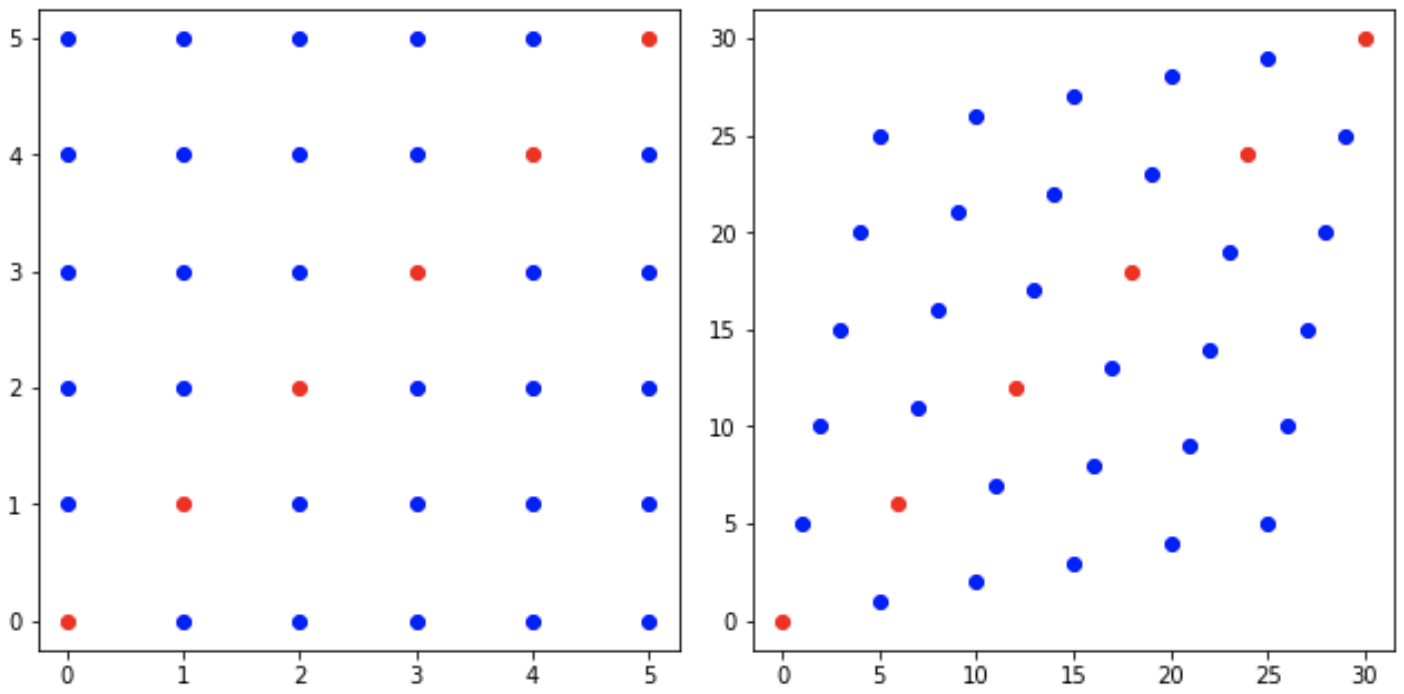
\includegraphics[width=0.75\textwidth]{eigenvectors}
\end{figure}

The fact that eigenvalues usually exist isn't totally obvious, and it's a fact that people can't shut up about.  If you remember one thing from linear algebra, it's probably eigenvalues.  But you cannot say that eigenvectors exist with some caveats (complex values, degenerate eigenspaces, square matrices).  We discuss these caveats in detail in section X.  However the SVD is analogous to eigenvalues, and requires no caveats.  We'll see throughout this book that for many applications of eigenvalues, the singular values produced by the SVD are sufficient.\footnote{We'll see in Section X that eigenvalues are needed to calculate the SVD, so we haven't obviated them entirely.}

To see why the SVD is analogous to eigenvectors, look at what $UDV^T$ does to a frame of the domain.  First $V^T$ rotates it, then $D$ stretches or squashes (or zeroes out) each axis.  (The standard basis elements are the eigenvectors of $D$.). Then the $U$ rotates the resulting stretched frame.  If anything, it's surprising that you can't get fixed axes by following the eigenvectors before and after the rotation.  We'll see in Section X how this can fail, and we'll talk in Section Y about the scenarios where it doesn't.

\subsection{Vectors and Covectors}

One view of matrices is that they're the product of vectors and covectors.  The columns of $A$ tell us how to act on standard basis vectors.  That is,

$$
A = 
\left[
  \begin{array}{cccc}
    \vertbar & \vertbar & & \vertbar \\
    |A_{*1}\rangle  & |A_{*2}\rangle & \cdots & |A_{*n}\rangle\rangle    \\
    \vertbar & \vertbar & & \vertbar 
  \end{array}
\right] =
\left[
  \begin{array}{cccc}
    \vertbar & \vertbar & & \vertbar \\
    A|e_1\rangle    & A|e_2\rangle   & \cdots & A|e_n\rangle    \\
    \vertbar & \vertbar & & \vertbar 
  \end{array}
\right]
$$

But any vector $\vec v=\begin{pmatrix} v_1  \\  v_2 \\ \vdots \\ v_n  \end{pmatrix}$ can be written as $|v\rangle = \sum_i v_i|e_i\rangle$.  So to figure out the effect of $A$ on $|v\rangle$, we only need to find the $i$-th component of $|v\rangle$ (i.e. $\langle e_i|v\rangle$ and multiple by $|A_{*1}\rangle$.  That is, $A=\sum_i|A_{*i}\rangle\langle e_i|$.

But in the course of studying linear algebra, you come to learn that there's nothing really special about the standard basis $\left\{|e_i\rangle\right\}$.  For any basis $\left\{| v _i\rangle\right\}$, we can write the matrix $A$ with this basis on the domain.  Call the columns of this new matrix $\left\{| u _i\rangle\right\}$, and it follows that $A=\sum_i| u _i\rangle\langle v _i|$.  Although $\left\{| v _i\rangle\right\}$ are orthonormal, it's not usually true of the resulting $\left\{| u _i\rangle\right\}$.  The existence of an SVD is the existence of a domain basis $\left\{| v _i\rangle\right\}$ for which the corresponding $\left\{| u _i\rangle\right\}$ are also orthogonal.  Pulling out the norms as $\lambda_i$ gives orthonormality.  Since there's no a priori reason to prefer one basis over another, the basis that SVD provides seems like a natural choice.  We'll see throughout the course of this book that it simplifies many things.

\subsection{Conventions}

The SVD yields a set of scalars $\left\{\lambda_i\right\}$ and vectors $\left\{\vec u_i, \vec v_i\right\}$.  We can and do require that all of these be real.  Throughout the book, we can mostly avoid talking about complex numbers.  An additional restriction that we impose in this book is that all the scalars be positive $\lambda_i>0$.  We can do this because if you had an SVD with a negative $\lambda_i$, then that summand $\lambda_i|u\rangle\langle v|=(-\lambda_i)|-u\rangle\langle v|$.  So we can call that form an SVD, but reject the one with negative coefficients.  As well if some $\lambda_i=0$, then that summand can be omitted.  Finally it will be convenient to order the singular values.  So we'll adopt the convention that these are ordered:  $\lambda_1\geq\lambda_2\geq\cdots\lambda_r$.  We prove in Section 3 that with our conventions, then multiset\footnote{By {\em multiset} we mean a collection where we care about the number of times each element appears, but we don't care about the order.} of scalars is unique to the matrix $A$; that is, it doesn't change based on different representations.  We may call these values the {\em singular values} of $A$.

Finally it will be convenient to order the singular values.  So we'll adopt the convention that these are ordered:  $\lambda_1\geq\lambda_2\geq\cdots\geq\lambda_r$.

\subsection{Outro}

The goal of this book is to build intuition and demonstrate applications.  With the intuition, the applications will seem natural.  (You should agree when you read Chapter 2.)  Hopefully by the end of the book, you'll be able to recall or modify the techniques more easily.  At this point, you should have some intuition for what an SVD is, but how somebody comes up with such a representation is still fairly abstract.  The rest of this chapter proves the existence and almost-uniqueness of the SVD.  Outside of these sections, this book generally is not heavy on the proofs.  But the techniques used in these proofs should help you get a concrete sense for what the SVD is.

{\bfseries\scshape\Large Exercises}

\begin{enumerate}[\thechapter.\thesection .1]
\item Continue the example from the beginning of the chapter, write $\left(
\begin{array}{ccc}
1 & 1 & 2 \\ 3 & 5 & 8
\end{array}
\right)$ in bra-ket form.  (Note: You should not have to recalculate anything.)
\item \label{rectangle_to_matrix_form} Given a matrix with SVD in bra-ket form:
$$
A=2\left(\begin{array}{c}1\\0\\0\end{array}\right)\left(\begin{array}{cc}1&0\end{array}\right) + 2\left(\begin{array}{c}0\\0\\1\end{array}\right)\left(\begin{array}{cc}0&1\end{array}\right)
$$
Write $A$ in matrix-form SVD two different ways.
\item A square matrix has an SVD $A=UDV^T$, with $D=\left(\begin{array}{cccc}\lambda_1&&&\\&\lambda_2&&\\&&\ddots&\\&&&\lambda_r\end{array}\right)$.  Show that all $\lambda_i\neq0$.  Next argue that $D^{-1}=\left(\begin{array}{cccc}\frac{1}{\lambda_1}&&&\\&\frac{1}{\lambda_2}&&\\&&\ddots&\\&&&\frac{1}{\lambda_r}\end{array}\right)$.  Finally prove that $A^{-1}=VD^{-1}U^T$.
\item \label{null_space_ex} Given a matrix with SVD $A=\sum_i\lambda_i|u_i\rangle\langle v_i|$, prove that $A\vec v=0$ if and only if $\vec v$ is perpendicular to each $\vec v_i$.
\item \label{range_ex} Given a matrix with SVD $A=\sum_i\lambda_i|u_i\rangle\langle v_i|$, prove that a vector $\vec u$ equals $A\vec v$ for some $\vec v$ if and only if $\vec u\in\operatorname{span}\left(\vec u_i\right)$.
\item The orthonormality of $U$ and $V$ will often be useful.  Given an SVD $A=\sum_i\lambda_i|u_i\rangle\langle v_i|$, verify the following.
\begin{enumerate}
\item For $|v\rangle = \sum_ia_i|v_i\rangle$, $A|v\rangle=\sum_ia_i\lambda_i|u_i\rangle$.
\item $\langle u_i|A|v_i\rangle=\lambda_i$.
\end{enumerate}
\end{enumerate}

\section{Existence}

In this section, we prove the existence of an SVD.  This proof is constructive, in the sense that it gives an algorithm for building a bra-ket form of an SVD.

\begin{algorithm}
\caption{SVD of a matrix $A$ of rank $r$.}
\label{alg1}
\begin{algorithmic}
\State $A_0 \gets A$
\While{$A_i\neq 0$}
	\State Find the unit vectors $\vec u _i$ and $\vec v _i$ that maximize\footnote{The keen-eyed mathematician may object that maximums don't always exist.  But because we've restricted to unit vectors, this is compact.  Therefore maximums exist.} $\langle u _i|A_{i-1}| v _i\rangle$.
	\State Set $A_i = A_{i-1}-| u _i\rangle\langle u _i|A| v _i\rangle\langle v _i|$
\EndWhile
\end{algorithmic}
\end{algorithm}

When the algorithm finishes, we have $A_r=0$.  So that $0=A_r=A-\sum_{i=1}^r| u _i\rangle\langle u _i|A_{i-1}| v _i\rangle\langle v _i|$.  We recognize that $\lambda_i:=\langle u _i|A_{i-1}| v _i\rangle$ is just a scalar, and add these to both sides so that we get $A=\sum_{i=1}^r\lambda_i| u _i\rangle\langle v _i|$.  The resulting vectors are normal, by choice.  But for this to be an SVD as described in the first section, we need the vectors $\left\{u_i\right\}_i$ to be a perpendicular set, and for $\left\{v_i\right\}_i$ to be a perpendicular set.  We prove that this is so in Theorem \ref{svd_perpendicular}.

An objection to this algorithm may be that it only works if the while loop eventually terminates.  For the algorithm to work, it must be true that $A_r=0$ for some $r$.  In Theorem \ref{svd_terminates}, we show that for $A$ with dimension $m\times n$ this must happen within $\min(m, n)$ steps.

I will spend the rest of the section proving that these are true.  But first, why does this work?  We see that $| u _i\rangle\langle u _i|A| v _i\rangle\langle v _i|=\lambda_i| u _i\rangle\langle v _i|$ is just a matrix that's the same shape as $A_{i-1}$.  But this is also the matrix that captures all of info from these two axes.  To see what this means, let's first look at a lower-dimensional analogy.

\begin{tcolorbox}[title=Example: Covector Analogy,colback=blue!5]
Consider the covector $v=\left(\begin{array}{ccc} 3 & 3 & 2 \end{array}\right)$.  If we wanted to remove all the signal along the axis $\left(\begin{array}{ccc} 1 \\ 0 \\ 0 \end{array}\right)$, then we would subtract $\left(\begin{array}{ccc} 3 & 0 & 0 \end{array}\right)$ from $v$ to get $\left(\begin{array}{ccc} 0 & 3 & 2 \end{array}\right)$.  Now any vector along that axis $\left(\begin{array}{c} \lambda \\ 0 \\ 0 \end{array}\right)$  gets zeroed out $\left(\begin{array}{ccc} 0 & 3 & 2 \end{array}\right)\left(\begin{array}{c} \lambda \\ 0 \\ 0 \end{array}\right) = 0$.  We got the $3$ when subtracting by looking at the first element, but this can be formalized as $3=\langle v|e_1\rangle$, where $|e_i\rangle$ is the vector with all zeroes and a single one at index $i$.  Now we can repeat this with the second dimension $3=\langle v|e_2\rangle$.  So now $v-3\langle e_1|-3\langle e_2| = \left(\begin{array}{ccc} 0 & 0 & 2 \end{array}\right)$.  This covector equals zero when it pairs with {\em any} linear combination of $|e_1\rangle$ and $|e_2\rangle$.  That is $\left(\begin{array}{ccc} 0 & 0 & 2 \end{array}\right)\left(\begin{array}{c} \lambda \\ \mu \\ 0 \end{array}\right) = 0$.  We can do an SVD-like algorithm to assign $v$'s signal to it's components: $v = \sum_{i=1}^3\langle v|e_i\rangle\langle e_i|$.  There's nothing special about the standard vectors.  It's true that for any basis $\left\{ v _i\right\}_{i=1}^3$, $\langle v| = \sum_{i=1}^3\langle v| v _i\rangle\langle v _i|$.  It's further true that if we stop short, the covector zeros out encountered vectors, like $\left(v-\langle v| v _1\rangle\langle v _1|-\langle v| v _2\rangle\langle v _2|\right)\left(\lambda| v _1\rangle+\mu| v _2\rangle\right)=0$.  We say that $\langle v| v _i\rangle\langle v _i|$ "captures all the info" from $\langle v|$ in the direction of $\langle v _i|$, because when subtract off that bit, there's nothing left in that direction.

So what we're doing with the covectors generalizes to the SVD algorithm we propose above.  We say that $| u \rangle\langle u |A| v \rangle\langle v |$ captures all the info from  $A$ in the direction of $ u $ and $ v $, because $\langle u |\left(A-| u \rangle\langle u |A| v \rangle\langle v |\right)| v \rangle=0$.  (Check that this is true.)  This isn't a proof yet, but this is why we think to try this.  By choosing the maximizing pair of vectors for remaining signal with each step, we guarantee that we're getting perpendicular vectors from earlier vectors.  The reasoning is that if we chose some vector that was pointing in a similar direction as an earlier vector, then we'd be pointing partly in a zeroing direction.  The zeroing part of the new matrix, $| u \rangle\langle u |A| v \rangle\langle v |$, starts by projecting onto the zeroed axis; if this projection is non-zero, then some part of the vector is going to waste.
\end{tcolorbox}

\subsection{Proof of the Correctness of Algorithm \ref{alg1}}

\begin{lemma}
\label{tollbooth}
For any matrix $A$, if $\langle u |A| v \rangle=\max_{\|u_i\|=\|v_i\|=1}\langle u_i |A| v_i \rangle$, then $A| v \rangle=\lambda| u \rangle$, for some scalar $\lambda$.
\end{lemma}

\begin{proof}
Fix the maximizing $|v\rangle$.  $A| v \rangle$ maps to some vector.  We call this vector $\lambda|t\rangle$, where $|t\rangle$ is a unit vector.  (The magnitude has been factored out into the scalar $\lambda$.  So $\langle t |A| v \rangle=\lambda\langle u | t\rangle$.  Given that $\langle u |$ and $| t\rangle$ are unit vectors, the inner product is given by the cosine of the angle between them (Theorem \ref{cos_sim}), which is maximized when the vectors are the same.
\end{proof}

This is an important fact, not only because it helps us in the next lemma, but also because it advances our intuition.  When we think of a matrix $A$ as a product of vectors and covectors, then we think of it as repeatedly projecting onto axes (covectors) and using those coefficients to determine how far to go in a certain direction (vectors).  This lemma says that when we've chosen the maximizing unit vector ($ u $) and covector ($ v $), as prescribed by the SVD algorithm, we've chosen a matching pair.  So that if we wanted to remove the effect of the projecting onto $ v $, then we need to subtract from the output some multiple of $ u $.

Note that though Lemma \ref{tollbooth} doesn't make a claim about the value of $\lambda$, it's easy to see that $\lambda=\langle u |A| v\rangle$, because $\langle u|A|v\rangle = \lambda\langle u|u\rangle = \lambda$.

Next we use this fact to see:

\begin{lemma}
\label{a1lemma}
Given $A_1=A-\lambda_1| u _1\rangle\langle v _1|$, then $A_1| v _1\rangle\langle v _1|=0$.
\end{lemma}

\begin{proof}
$$
\begin{array}{rcll}
A_1| v _1\rangle\langle v _1| &=& \left(A-\lambda_1| u _1\rangle\langle v _1|\right)| v _1\rangle\langle v _1|& \\
&=& A| v _1\rangle\langle v _1| - \lambda_1| u _1\rangle\langle v _1| v _1\rangle\langle v _1| & \quad\text{Distribute}\\
&=& \left(A| v _1\rangle\right)\langle v _1| - \lambda_1| u _1\rangle\langle v _1|& \\
&=& \left(\lambda_1| u _1\rangle\right)\langle v _1| - \lambda_1| u _1\rangle\langle v _1|&\quad\text{By Lemma \ref{tollbooth}} \\
&=& 0
\end{array}
$$
\end{proof}

We can immediately conclude from Lemma \ref{a1lemma} that $A_1=A_1\left(I-| v _1\rangle\langle v _1|\right)$.  This says that applying $A_1$ to a vector $| v \rangle$ is the same as first applying $\left(I-| v _1\rangle\langle v _1|\right)$ to $| v \rangle$, then applying $A_1$ to the resulting vector.  $\left(I-| v _1\rangle\langle v _1|\right)$ is a special matrix that acts on any vector by projecting onto the subspace of all vectors perpendicular to $| v _1\rangle$.  This will be justified reach the section on projection matrices.  For now it's sufficient to understand:

\begin{enumerate}
\item  $\left(I-| v _1\rangle\langle v _1|\right)| v \rangle$ is exactly $| v \rangle$ when $\langle v _1| v \rangle=0$.  I.e. $ v $ is perpendicular to $ v _1$, and 
\item  $\left\Vert\left(I-| v _1\rangle\langle v _1|\right)| v \rangle\right\Vert < 1$, otherwise.
\end{enumerate}

The first statement is obvious.  The second statement should be fairly intuitive because we're subtracting off a component of a vector.  This is analogous to zeroing out the first term of a unit vector, which will leave it smaller.  A more formal proof of this point is left as Exercise \ref{finish_projection}.

We state without justification that this also holds for more vectors.  This fact follows in much the same way as single case we've discussed, but the proof is tedious.

 \begin{theorem}
\label{lil_projection_thm}
For $A_i$ as defined above,
\begin{enumerate}
\item $A_i| v \rangle=A_i\left(I-\sum_{k=1}^{i-1}| v _k\rangle\langle v _k|\right)| v \rangle$
\item $\left\Vert\left(I-\sum_{k=1}^{i}| v _k\rangle\langle v _k|\right)| v \rangle\right\Vert<1$ unless $| v \rangle$ is perpendicular to each of the earlier $| v _k\rangle$
\end{enumerate}
 \end{theorem}

Finally because the same logic can be done on the other side of the matrix, we have $A_i=\left(I-\sum_{k=1}^i| u _k\rangle\langle u _k|\right)A_i$.  So we make a more general statement.

\begin{corollary}
\label{double_side_proj}
For $A_i$ as defined above,
$$
A_i=\left(I-\sum_{k=1}^i| u _k\rangle\langle u _k|\right)A_i\left(I-\sum_{k=1}^{i-1}| v _k\rangle\langle v _k|\right)
$$
\end{corollary}

We're ready to prove the theorems mentioned at the opening of this chapter.  First we'll prove that the vectors $\left\{\langle u_i|\right\}$ are perpendicular, and that $\left\{|v_i\rangle\right\}$ are perpendicular.  Specifically we argue that each new vector generated by the algorithm is perpendicular to all previous ones.

 \begin{theorem}
Let $A_i$ be as in Algorithm \ref{alg1} with $A_i\neq0$.  If $u_i$, $v_i$ maximize $\langle u |A_i| v \rangle$, then $u_i$ is perpendicular to $u_j$ and $v_i$ is perpendicular to $v_j$ for all $j<i$.
 \end{theorem}

\begin{proof}
\label{svd_perpendicular}
Suppose to the contrary that one or both of the vectors is not perpendicular, and that the maximum is $M$.

$M$ must be positive.  $\langle u|A|v\rangle$ must be non-zero for at least one pair of vectors, for otherwise $A_i=0$.  Consider a non-zero value, $\langle u|A|v\rangle$.  If it's positive, then the maximum, $M$ must be positive.  Otherwise $\langle -u|A|v\rangle$ must be positive, which implies $M>0$.

Using Corollary \ref{double_side_proj}, we can write $M$ as:

$$
M=\langle u |A_i| v \rangle=\langle u |\left(I-\sum_{k=1}^i| u _k\rangle\langle u _k|\right)A_i\left(I-\sum_{k=1}^{i}| v _k\rangle\langle v _k|\right)| v \rangle=\langle u '|A_i| v '\rangle
$$

where $\langle u'|=\langle u |\left(I-\sum_{k=1}^i| u _k\rangle\langle u _k|\right)$ and $|v'\rangle=\left(I-\sum_{k=1}^{i}| v _k\rangle\langle v _k|\right)| v \rangle$.

Because we assumed that either $\vec u$ or $\vec v$ are not perpendicular to all previous vectors, one of vectors $ u '$ or $ v '$ have magnitude less than $1$, by Theorem \ref{lil_projection_thm}, point (b).

We can now reach a contradiction, because the unit vectors $\frac{\langle u '|}{\left\Vert\langle u '|\right\Vert}$ and $\frac{| v '\rangle}{\left\Vert| v '\rangle\right\Vert}$ do a better job of maximize $\langle u|A|v\rangle$ than $\langle u_i|$ and $|v_i\rangle$.  This is because:

$$
\frac{\langle u '|}{\left\Vert\langle u '|\right\Vert}A_i\frac{| v '\rangle}{\left\Vert| v '\rangle\right\Vert} = \frac{\langle u'|A_i|v'\rangle}{\left\Vert\langle u '|\right\Vert\left\Vert| v '\rangle\right\Vert} = \frac{M}{\left\Vert\langle u '|\right\Vert\left\Vert| v '\rangle\right\Vert} > M >0
$$

\end{proof}

Finally we prove that Algorithm \ref{alg1} terminates.

 \begin{theorem}
\label{svd_terminates}
If $A$ is dimension $m\times n$, call $r:=\min(m,n)$, then $A_r=0$.
 \end{theorem}

Note:  This doesn't preclude $A_{r'}=0$ for some $r'<r$.  If that happens, then the algorithm will terminate early.

\begin{proof}
Suppose we've gone through $r$ steps, then it must be that the set of perpendicular covectors $\left\{\langle u _i|\right\}$ span the codomain {\em or} the set of perpendicular vectors $\left\{| v _i\rangle\right\}$ span the domain, depending on if $r=m$ or $r=n$.  Without loss of generality, say that the domain is spanned.  Then 
$$
\begin{array}{rcll}
A_r&=&A_r\left(I-\sum_{i=1}^{r'}| v _i\rangle\langle v _i|\right)&\quad\text{by Theorem \ref{lil_projection_thm}}\\
&=&A0&\quad\text{by Exercise \ref{outer_product_identity}}\\
&=&0&
\end{array}
$$
\end{proof}

\subsection{Change of bases for outer product sums}

Before moving on, we'll state a fact that we'll need later.  This is a little out of place here, except that it shows a nice application of the concepts cover in this section.

We saw in Exercise X that for any basis $\left\{|v_i\rangle\right\}$, we have $\sum_i|v_i\rangle\langle v_i|$.  And a natural extension of this is that if you had two sets of orthonormal vectors, $\left\{|v_i\rangle\right\}$ and $\left\{|v_i'\rangle\right\}$, then $\sum_i|v_i\rangle\langle v_i|=\sum_i|v_i'\rangle\langle v_i'|$.  Basically this says that for summations of these $|v_i\rangle\langle v_i|$, it only really matters what space you're spanning; you're free to change basis however you want.  This turns out to be true, but we won't prove it here, because we actually need something a little more general.  We will encounter in the next section these sums of outer products, but they won't be necessarily symmetric.  So we need that $\sum_i|u_i\rangle\langle v_i|=\sum_i|u_i'\rangle\langle v_i'|$.  This only happens under special circumstances, but these happen to be the circumstances that arise when picking apart the SVD.

\begin{lemma}
\label{rebase_projections}
For orthonomal sets of vectors $\left\{\langle u_i|\right\}_{i=1}^n$, $\left\{|v_i\rangle\right\}_{i=1}^n$, $\left\{\langle u_i'|\right\}_{i=1}^n$, and $\{|v_i'\rangle\}_{i=1}^n$, we have
$$
\sum_i|u_i\rangle\langle v_i|=\sum_i|u_i'\rangle\langle v_i'|
$$
If the following conditions hold:
\begin{enumerate}
\item $\operatorname{span}\left\{\langle u_i|\right\}=\operatorname{span}\left\{\langle u_i'|\right\}$ and $\operatorname{span}\left\{|v_i\rangle\right\}=\operatorname{span}\left\{|v_i'\rangle\right\}$.
\item There exists a fixed linear map $B$ such that $B|v_i\rangle=|u_i\rangle$ and $B|v_i'\rangle=|u_i'\rangle$.
\end{enumerate}
\end{lemma}

For the second point, there will always exist some mapping from one orthonormal set to another (of the same cardinality).  The key assumption here is that the $B$ is the same between the pairs of sets.

\begin{proof}
Call $M=\sum_i|u_i\rangle\langle v_i|$ and $M'=\sum_i|u_i'\rangle\langle v'|$.  To prove these matrices are equal, we they act the same on every vector.  We chose some arbitrary vector $|v\rangle$, and show that $M|v\rangle=M'|v\rangle$.

By Theorem \ref{vector_decomp}, we can write $|v\rangle=|v_\parallel\rangle+|v_\bot\rangle$ with $W$ in the Theorem set as $\operatorname{span}\left\{|v_i\rangle\right\}=\operatorname{span}\left\{|v_i'\rangle\right\}$.  With this construction $\langle v_i|v_\bot\rangle=0$ for each $\langle v_i|$, so $M|v_\bot\rangle=M'|v_\bot\rangle=0$.

Because $|v_\parallel\rangle\in\operatorname{span}\{|v_i\rangle\}$, $|v_\parallel\rangle=\sum_ia_i|v_i\rangle$.

$$
\begin{array}{rcl}
M|v\rangle &=& M|v_\parallel\rangle+M|v_\bot\rangle \\
 &=& M|v_\parallel\rangle \\
 &=& \left(\sum_i|u_i\rangle\langle v_i|\right)\left(\sum_ja_j|v_j\rangle\right) \\
 &=& \sum_i|u_i\rangle a_i \\
 &=& \sum_ia_iB|v_i\rangle \\
 &=& B\left(\sum_ia_i|v_i\rangle\right) \\
 &=& B|v_\parallel\rangle
\end{array}
$$

The same calculation with primes on all the $M$, $u$, and $v$ variables gives that $M'|v\rangle$ also equals $B|v_\parallel\rangle$.  
\end{proof}

{\bfseries\scshape\Large Exercises}

\begin{enumerate}[\thechapter.\thesection .1]
\item \label{finish_projection} Given unit vectors $u$ and $v$.  Prove that if $\langle u|v\rangle\neq0$, then $\left\Vert\left(I-|u\rangle\langle u|\right)|v\rangle\right\Vert < 1$.  (Hint:  For any vector $ v $, $\Vert  v \Vert<1$ if and only $\langle  v | v \rangle<1$.)
\item \label{outer_product_identity} Given a basis $\left\{\vec v_i\right\}_{i=1}^n$ of $\mathbb R^n$, prove that $I=\sum_{i=1}^n|v_i\rangle\langle v_i|$.
\item Given a matrix with a SVD $A=\sum_i\lambda_i|u_i\rangle\langle v_i|$, show that $A=\sum_i\langle v_i| A^T\langle v_i|$.  (Hint: Use Lemma \ref{a1lemma}.)
\end{enumerate}

\section{Almost Uniqueness}\label{almost_uniqueness}

An annoying fact about the SVD is that it's not unique.  But it turns out to be {\em almost} unique.  In this section, we see that there are limitations.

Let's review briefly.  Given a matrix $A$, we can find a SVD, $A=\sum_i\lambda_i|u_i\rangle\langle v_i|$.  The $\lambda_i$ do not need to be distinct.  For the sake of this section, we write this as 

\begin{equation}
\label{multilambda}
A=\sum_i\lambda_i\sum_{j=1}^{n_i}|u_{ij}\rangle\langle v_{ij}|,
\end{equation}

 where $\lambda_1>\lambda_2>\cdots$.  By indexing the vectors/covectors with a second index $j$, we can make sure that all our $\lambda_i$ are unique.
 
\begin{tcolorbox}[title=Example,colback=blue!5]
Suppose we had an SVD:
$$
A=2|u_1\rangle\langle v_1|+2|u_2\rangle\langle v_2|+2|u_3\rangle\langle v_3|+|u_4\rangle\langle v_4|+|u_5\rangle\langle v_5|
$$

To rewrite this in the language of Equation (\ref{multilambda}), we would write:
$$
A=2\cdot\left(|u_{11}\rangle\langle v_{11}|+|u_{12}\rangle\langle v_{12}|+|u_{13}\rangle\langle v_{13}|\right)+1\cdot\left(|u_{21}\rangle\langle v_{21}|+|u_{22}\rangle\langle v_{22}|\right)
$$

So that $\lambda_1=2$ and $\lambda_2=1$.  $|u_1\rangle$ gets renamed to $|u_{11}\rangle$, $\langle v_4|$ gets remapped to $\langle v_{21}|$, etc.

\end{tcolorbox}

If the SVD was built with our algorithm from the previous section, then $\langle u_{11}|A|v_{11}\rangle=\lambda_1$ maximizes $\langle u|A|v\rangle$.  Of course because $\langle u_{1j}|A|v_{1j}\rangle=\lambda_1$ for any $1\leq j\leq n_i$, the algorithm may just have chosen $u_{1,2}$ or $u_{1,3}$ first, so any reordering of these could have been produced.  In fact we don't need to be restricted to these exact vectors; for {\em any} unit vector $|v\rangle\in\operatorname{span}\left\{|u_{i*}\rangle\right\}$, we can find a $\langle u|$ (given by Lemma \ref{a1lemma}) for which $\langle u|A|v\rangle=\lambda_1$.  It also turns out that any $|v\rangle\not\in\operatorname{span}\left\{|v_{i*}\rangle\right\}$, there is not a $\langle u|$ for which $\langle u|A|v\rangle=\lambda_1$.  These two statements are proven in Corollary \ref{corollary1}.

Together these show that if you follow the algorithm from the previous section of repeatedly finding the maximizing vectors, the only variation you can get is a change of basis in $|v_{i*}\rangle$.  (If $n_i=1$, then this means that we can only vary $\lambda_1|u\rangle\langle v|=\lambda_1|-u\rangle\langle -v|$.)  Actually we've only shown this for for the largest $\lambda=\lambda_1$, but by subtracting off these components and applying the same argument to the resulting difference with a new largest $\lambda=\lambda_2$, we can apply the same argument; this is a trick we'll use repeatedly.

So running the algorithm won't give you the exact same answer each time you do it.  It may vary, but only in choosing different a different basis for each $\left\{|v_{i*}\rangle\right\}$.  But is it possible to use some other algorithm to come up with a SVD?  And maybe if you did, you'd get a much different SVD?  We show in this section that no matter how you come up with an SVD it must be the same as one of the SVDs created by the algorithm.  That is, it can only vary by a change of basis for each spanning space $\operatorname{span}\left\{\langle u_{i*}|\right\}$ and $\operatorname{span}\left\{|v_{i*}\rangle\right\}$.

 \begin{theorem}
\label{upperbound}
Given an SVD of a matrix, $A=\sum_i\lambda_i|u_i\rangle\langle v_i|$, then for any $\vec u$, $\vec v$, $\langle u|A|v\rangle\leq\lambda_1$.
 \end{theorem}

\begin{proof}
Rearranging Lemma \ref{a1lemma}, we get that

$$
\max_{\|u\|=\|v\|=1}\langle u|A|v\rangle = \max_{\|v\|=1} \frac{\langle v|A^TA|v\rangle}{\left\|A|v\rangle\right|}
$$

For any vector $\vec w$, $\left\|\vec w\right\|=\sqrt{\vec w^T\vec w}$.  So,

$$
\max_{\|v\|=1} \frac{\langle v|A^TA|v\rangle}{\left\|A|v\rangle\right\|}
= \max_{\|v\|=1} \frac{\langle v|A^TA|v\rangle}{\sqrt{\langle v|A^TA|v\rangle}}
= \max_{\|v\|=1} \sqrt{\langle v|A^TA|v\rangle}
$$

A common trick is to notice that the square root of a value is maximal exactly when the value itself is maximal.  So that the same $|v\rangle$ that maximizes $\langle u|A|v\rangle$ also maximizes $\langle v|A^TA|v\rangle$.

So to maximize $\langle v|A^TA|v\rangle$, we use the fact that $A^TA=\sum_i\lambda_i^2|v_i\rangle\langle v_i|$ (Lemma \ref{ata_eq}).  If $\left\{\vec v_i\right\}$ do not span the domain (with dimension $=n$), then we pad it with additional basis vectors, and $\lambda_i=0$.  $A^TA=\sum_{i=1}^n\lambda_i^2|v_i\rangle\langle v_i|$.  Now $\left\{\vec v_i\right\}_{i=1}^n$ is a basis so that any unit vector $|v\rangle = \sum_{i=1}^na_i|v_i\rangle$, with $\sum_{i=1}^na_i^2 =1$.

\begin{equation}
\label{upperbound_eqn}
\begin{array}{rcl}
\langle v|A^TA|v\rangle &=& \langle v|\left(\sum_i\lambda_i^2|v_i\rangle\langle v_i|\right)|v\rangle \\
 &=& \left(\sum_i a_i\langle v_i|\right)\left(\sum_i\lambda_i^2|v_i\rangle\langle v_i|\right)\left(\sum_i a_i|v_i\rangle\right) \\
 &=& \sum_ia_i^2\lambda_i^2 
 \leq \sum_ia_i^2\lambda_1^2 
 = \lambda_1^2
\end{array}
\end{equation}

The inequality on the last line follows because $\lambda_1$ is larger than all the other $\lambda_i$.
\end{proof}

Notice, that by eliminating the $\langle u|$, the problem of maximizing became easier.  After finding $|v\rangle$, we could use Lemma \ref{a1lemma} to find $\langle u|$.  But by symmetry, we could have instead found the $\langle u|$ that maximizes $\langle u|AA^T|u\rangle$.

While the theorem gives an upper bound of $\lambda_1$, note that this bound is achievable, namely with $\vec u_1$ and $\vec v_1$.  But we can be a little more specific:

\begin{corollary}
\label{corollary1}
Given a matrix with SVD, $A=\sum_i\lambda_i\sum_{j=1}^{n_i}|u_{ij}\rangle\langle v_{ij}|$ (with $\lambda_1>\lambda_2>\cdots$) and a unit vector $|v\rangle$, $\max_{\|u\|=1}\langle u|A|v\rangle=\lambda_1$ if and only if $|v\rangle\in\operatorname{span}\left\{|v_{i*}\rangle\right\}$.
\end{corollary}

We skip some of the details to this proof.  It amounts to observing that the equality at the end of Eq. (\ref{upperbound_eqn}) is strict unless all the non-zero terms have $\lambda_i$ coefficients equal to $\lambda_1$.

\begin{proof}
Redo the work of Lemma \ref{ata_eq}, but this time with the SVD written as $A=\sum_i\lambda_i\sum_{j=1}^{n_i}|u_{ij}\rangle\langle v_{ij}|$ to get

$$
A^TA=\sum_i\lambda_i\sum_{j=1}^{n_i}|v_{ij}\rangle\langle v_{ij}|
$$

By the same steps logic as Eq. (\ref{upperbound_eqn}), we get that

$$
\langle v|A^TA|v\rangle = \sum_ia_i^2\lambda_i^2
$$

where $a_i^2=\sum_ja_{ij}^2$, with $a_{ij}$ the coefficient of $|v_{ij}\rangle$ in the decomposition of $|v\rangle$.  Again we have that the coefficients must satisfy $\sum_ia_i^2=1$, but this time the coefficients are distinct, so it's clear that this equals $\lambda_1$ if and only if $a_1=$ and all others are $0$.  But this happens if and only if $|v\rangle\in\operatorname{span}\left\{|v_{1*}\rangle\right\}$.

\end{proof}

Some words should be said about Theorem \ref{upperbound} and Corollary \ref{corollary1}.  We'll see in a bit that this is used to prove the almost-uniqueness of the SVD.  In many ways, this Theorem \ref{upperbound} are the keystone of the entire chapter; it connects all the concepts.  Though it depends on the existence of an SVD, we now see a motivation for Algorithm \ref{alg1}:  The first singular value $\lambda_1$ is something fundamental about the matrix - it doesn't depend on the SVD representation.  So it make sense that we should try to obtain it, and Theorem \ref{upperbound} shows that you obtain it by pulling by maximizing $\langle u|A|v\rangle$.  The next chapter shows how to calculate the vectors $|v_i\rangle$.  That calculation relies entirely on this trick (first encountered in Theorem \ref{upperbound}) of canceling the $\langle u_i|$ by taking $A^TA$.

Theorem \ref{upperbound} and its corollary are also perhaps the most surprising.  It seems sort of like magic.  Maybe you're along for the ride when I said that we'll take $A^TA$ to cancel out the $|u_i\rangle$, but it seems like luck when the you end up with $\sum_ia_i^2$, which just happened to be $1$, by nature of looking at unit vectors.  Maybe there's some magic here.  But at the same time, matrices are sometimes thought of as quadratic operators.  For a vector $\vec x=\left(\begin{array}{c}x_1\\x_2\\\vdots\\x_n\end{array}\right)$ and an $n\times n$ matrix $M$, $\vec x^TM\vec x$ has every power-$2$ term of $x$ with coefficients derived from $M$.  (Check this.)  Given this quadratic nature, maybe it's less surprising that it'd take vector components to their magnitude.

Imagine that your matrix $A$ is a diagonal matrix.  This is already an SVD with $D=A$ and $U=V=I$.  Look at how obvious the logic here is now.  With some $\vec x=\left(\begin{array}{c}x_1\\x_2\\\vdots\\x_n\end{array}\right)$, $\langle x|D|x\rangle=\sum_i\lambda_ix_i^2$.  If you wanted the first singular value, $\lambda_1$, the largest value, then you need to do something to get $A_{11}$.  Of course $A_{11}=\langle e_1|A|e_1\rangle$ would do the trick.  When $U$ and $V$ aren't the identity then you should do $\langle e_1|U^T$ and $V|e_1\rangle$ to cancel.  The existence of the SVD just says that aside from these little twists, $U$ and $V^T$, all matrices are just these canonical quadratic forms.

With that digression behind us, we can now actually prove almost uniqueness.  All the hard work has been done already.  This theorem brings together lots of ideas, so take your time with it.

\begin{theorem}
Given two SVDs of a matrix $A=\sum_i\lambda_i\sum_{j=1}^{n_i}|u_{ij}\rangle\langle v_{ij}|=\sum_i\lambda_i'\sum_{j=1}^{n_i'}|u_{ij}'\rangle\langle v_{ij}'|$, then for each $i$:

\begin{enumerate}
\item $\lambda_i=\lambda_i'$
\item $n_i=n_i'$
\item $\operatorname{span}\left\{\vec u_{i*}\right\}=\operatorname{span}\left\{\vec u_{i*}'\right\}$
\item $\operatorname{span}\left\{\vec v_{i*}\right\}=\operatorname{span}\left\{\vec v_{i*}'\right\}$
\end{enumerate}
\end{theorem}

\begin{proof}

We first prove the four statements for $i=1$.

Theorem \ref{upperbound} tells us that the largest value of $\langle u|A|v\rangle$ is the largest singular value for any SVD.  Because these SVDs represent the same matrix, $A$, it follows that these two singular values are equal, $\lambda_1=\lambda_1'$.  So (1) is true.

Because $\langle u_{1j}|A|v_{1j}\rangle=\lambda_1=\lambda_1'$ for each $j$, Corollary \ref{corollary1} tells us that $\langle u_{1j}|\in\operatorname{span}\left\{\langle u_{1*}'|\right\}$ and $|v_{1j}\rangle\in\operatorname{span}\left\{|v_{1*}'\rangle\right\}$.  Since spans are closed under linear combinations, it follows also that $\operatorname{span}\left\{\langle u_{1*}|\right\}\subset\operatorname{span}\left\{\langle u_{1*}'|\right\}$ and $\operatorname{span}\left\{|v_{1*}\rangle\right\}\subset\operatorname{span}\left\{|v_{1*}'\rangle\right\}$.  Applying the same argument in the other direction, we get the subset going the other direction, so that by double inclusion, we can conclude that $\operatorname{span}\left\{\langle u_{1*}|\right\}=\operatorname{span}\left\{\langle u_{1*}'|\right\}$ and $\operatorname{span}\left\{|v_{1*}\rangle\right\}=\operatorname{span}\left\{|v_{1i*}'\rangle\right\}$.  This proves (3) and (4).

Because $\left\{|v_{1*}\rangle\right\}$ are orthonormal, the dimension of their span is the number of elements in the set, $n_1$.  The span of $\left\{|v_{1*}'\rangle\right\}$ is the same space, so the same dimension.  But this time the dimension is the number of elements in this orthonormal set, $n_1'$.  It follows that $n_1=n_1'$, which proves (2).

We've only proven this for the first singular value.  This is because Theorem \ref{upperbound} and Corollary \ref{corollary1} are only proven for the maximum singular value.  We want to use the usual trick of subtracting that signal out and repeating the argument on the resulting matrix, repeatedly.  Usually we gloss over this detail, but here requires a little more care.  We subtract $A-\lambda_1\sum_{j=1}^{n_i}|u_{ij}\rangle\langle v_{ij}|$.  On the representation $\sum_{i=1}^n\lambda_i\sum_{j=1}^{n_i}|u_{ij}\rangle\langle v_{ij}|$, this just removes the first summand.

$$
A-\lambda_1\sum_{j=1}^{n_i}|u_{ij}\rangle\langle v_{ij}|=\sum_{i=2}^n\lambda_i\sum_{j=1}^{n_i}|u_{ij}\rangle\langle v_{ij}|
$$

However for the other representation, we have something messier.

$$
A-\lambda_1\sum_{j=1}^{n_i}|u_{ij}\rangle\langle v_{ij}|=\lambda_1\left(\sum_{j=1}^{n_j}|u_{ij}'\rangle\langle v_{ij}'|-\sum_{j=1}^{n_j}|u_{ij}\rangle\langle v_{ij}|\right)+\sum_{i=2}^n\lambda_i'\sum_{j=1}^{n_i'}|u_{ij}'\rangle\langle v_{ij}'|
$$

In order to repeat the above argument, we need to reduce this to an SVD again.  We use Lemma \ref{rebase_projections} with $B=\frac{1}{\lambda_1}A$ to conclude that $\sum_{j=1}^{n_j}|u_{ij}'\rangle\langle v_{ij}'|=\sum_{j=1}^{n_j}|u_{ij}\rangle\langle v_{ij}|$, which cancels out the $\lambda_1$ terms from the above, resulting in:

$$
A-\lambda_1\sum_{j=1}^{n_i}|u_{ij}\rangle\langle v_{ij}|=\sum_{i=2}^n\lambda_i'\sum_{j=1}^{n_i'}|u_{ij}'\rangle\langle v_{ij}'|
$$

Now we have the two SVDs of $A-\lambda_1\sum_{j=1}^{n_i}|u_{ij}\rangle\langle v_{ij}|$, $\sum_{i=2}^n\lambda_i'\sum_{j=1}^{n_i'}|u_{ij}'\rangle\langle v_{ij}'|$ and $\sum_{i=2}^n\lambda_i\sum_{j=1}^{n_i}|u_{ij}\rangle\langle v_{ij}|$.  So we can repeat the above arguments on this.  Subtract, and repeat again, and so on.

\end{proof}

This tells you is that no matter how you obtain the SVD, it will be in basically the same form.  It will have the same singular values with the same multiplicity, and the only difference is that there may be a different basis chosen for the vectors.

This is a lot of work to show almost uniqueness, but by now we should start to have some intuition for what the SVD is.  Firstly, the singular values are something fundamental about the matrix, and not something that depends on the SVD representation.  Secondly, our algorithm from the previous section is a rational thing to try.  The largest singular value defines a space where these values can occur, but then after you subtract out that dimension, you get a big jump down to the next singular value.

{\bfseries\scshape\Large Exercises}

\begin{enumerate}[\thechapter.\thesection .1]
\item With an SVD given by Eq. (\ref{multilambda}), show that if $|v\rangle\in\operatorname{span}\{|v_{i*}\rangle\}$, then $A|v\rangle\in\operatorname{span}\{|u_{i*}\rangle\}$.
\item Given a matrix with SVD $A=\sum_i\lambda_i|v_i\rangle\langle v_i|$, show that for any $n\in\mathbb N$, $A^n=\sum_i\lambda_i^n|v_i\rangle\langle v_i|$.
\item Given a matrix with a SVD $A=\sum_i\lambda_i|u_i\rangle\langle v_i|$, show that $A=\left(\sum_i|u_i\rangle\langle u_i|\right)A\left(\sum_j|v_j\rangle\langle v_j|\right)$ by distributing the sums and arguing that $\langle u_i|A|v_j\rangle$ equals $\lambda_i$ if $i=j$ and $0$ otherwise.  How could you show this equality without distributing?
\item Given an invertible square matrix $A$ with minimum singular $\lambda_n$, prove that for any unit vectors $\vec u$ and $\vec v$, $\langle u|A|v\rangle\geq\lambda_n$.
\item Given a matrix $A$, prove that for any value $t$ between the smallest and largest singular value $\lambda_n\leq t\leq\lambda_1$, there are some unit vectors $\langle u|$ and $|v\rangle$ for which $\langle u|A|v\rangle=t$.
\end{enumerate}

\section{How to Calculate}

So far we haven't said how to actually calculate an SVD.  How to find the maximal vectors, as we've described.  In this section we show that this calculation amounts to calculating certain eigenvalues and eigenvectors.  In practice, you could calculate the SVD using a computer program.  (See Section \ref{computer_section}.)  Even though we can use computers, knowing how to calculate manually will advance our understanding of the SVD.

Before going on, we need a small fact about calculus.  I'll state a lemma here without proof.  Calculus is outside the scope of this book, but I provide some discussion in Appendix X.

\begin{lemma}
\label{calc}
For any square matrix $B$,

$$
\frac{\partial}{\partial|v\rangle}\langle v|B|v\rangle = 2B|v\rangle
$$
\end{lemma}

The right hand side of this equation is a vector whose entries equal $\frac{\partial\langle v|B|v\rangle}{\partial v_i}$.  This lemma seems simple.  (It's analogous to $d(bx^2)=2x$.). Indeed, it could be demonstrated with basic calculus, but the calculation is slightly more difficult than you may guess.

We saw in the last section that we could find $|v_1\rangle$ in $A=\sum_i\lambda_i|u_i\rangle\langle v_i|$ as the unit vector $|v\rangle$ that maximizes $\langle v|A^TA|v\rangle$.  To calculate this max, we can do some calculus, but we have to be careful to restrict to unit vectors ($\langle v|v\rangle=1$).  To enforce this, we use Lagrange multipliers.  (We call the Lagrange multiplier $\varepsilon$ instead of the usual $\lambda$ to avoid confusion with singular values.)

$$
\langle v|A^TA|v\rangle-\lambda\langle v|v\rangle=\langle v|\left(A^TA-\varepsilon I\right)|v\rangle
$$

By taking the derivative using Lemma \ref{calc} and setting to zero, we get

$$
\left(A^TA-\varepsilon I\right)|v_1\rangle=0
$$

That is, $|v\rangle_1$ is an eigenvector of $A^TA$.  Though this doesn't tell us which eigenvector, we can check all eigenvectors until we get a maximum.  Similarly $|u_1\rangle$ is an eigenvector of $AA^T$.

If the eigenvalue corresponding to $|v_1\rangle$ is $\varepsilon_1$, then $\langle v_1|A^TA|v_1\rangle=\varepsilon_1$.  From the discussion in the proof of Theorem X,

$$
\lambda_1=\langle u_1|A|v_1\rangle=\sqrt{\langle v_1|A^TA|v_1\rangle}=\sqrt{\varepsilon_1}
$$

It's not surprising that these vectors are eigenvectors of $A^TA$, because recall that 

$$
A^TA=\sum_i\lambda_i^2|v_i\rangle\langle v_i|.
$$

It's clear to see that $A^TA|v_i\rangle=\lambda_i^2|v_i\rangle$, which makes it an eigenvector.

Yet another way to see this to write $A=UDV^T$, so that $A^TA=VD^2V^T$.  Because $V^T$ rotates the domain.  You can see this as a rotation, a stretch or squeeze along the axes, then a rotation back ($V$).  $V^T$ maps each of the vectors $\vec v_i$ to the axes, and $V$ maps the axes back to the vectors $\vec v_i$.  It clear to see then that $VD^2V^T$ maps each $\vec v_i$ to some $\varepsilon_i\vec v_i$.

{\bfseries\scshape\Large Exercises}

\begin{enumerate}[\thechapter.\thesection .1]
\item Using the eigenvector technique presented in this section, calculate the SVD of $\left(\begin{array}{cc}2&6\\1&1\end{array}\right)$.
\item Prove that the eigenvalues of $A^TA$ form the same multiset as the eigenvalues of $AA^T$.
\item Show that for any $j>i$ an eigenvector corresponding to a non-zero eigenvalue of $A_j$ is also an eigenvector of $A_i$.
\item Given a symmetric matrix $A$ with distinct singular values, prove that every SVD has the form $\sum_i\lambda_i|v_i\rangle\langle v_i|$.
\end{enumerate}

\section{Quick Conclusions}

Though it took a lot of work to build some understanding of the SVD, we will use it throughout the book.  Next chapter, we can discuss a number of applications of the SVD.  For now, I will whet your appetite with some immediate conclusions.

\subsection{Rank-Nullity Theorem}

 \begin{theorem}
If $A$ is an $m\times n$-dimensional matrix, then $\operatorname{Dim}\left(\operatorname{Range}(A)\right)+\operatorname{Dim}\left(\operatorname{NullSpace}(A)\right)=n$.
 \end{theorem}

\begin{proof}
Choose some SVD of $A=\sum_{i=1}^r|u_i\rangle\langle v_i|$.  Expand $\left\{|v_i\rangle\right\}_{i=1}^r$ to a basis of the domain by adding vectors $|v_{r+1}\rangle, |v_{r+2}\rangle, ..., |v_n\rangle$.  Clearly $\operatorname{Range}(A)=\operatorname{Span}\left\{\langle u_i|\right\}_{i=1}^r$.  And $\operatorname{NullSpace}(A)=\operatorname{Span}\left\{|v_i\rangle\right\}_{i=r+1}^n$.  (See Exercises \ref{null_space_exercise} and \ref{range_exercise}.)  So the equality follows.
\end{proof}

\subsection{Determinant}

 \begin{theorem}
Let $A$ be an $m\times m$-dimensional matrix with $m$ (not-necessarily-distinct) singular values, $\lambda_1, ..., \lambda_m$.  Then $|A|=\prod_{i=1}^n\lambda_i$.
 \end{theorem}

\begin{proof}
Choose an SVD, $A=UDV^T$.  Because determinant distributes over matrix multiplication, $|A|=|U|\cdot|D|\cdot|V^T|$.  Because they're orthogonal, $|U|=|V^T|=1$.  So $|A|=|D|$.  $D$ is a diagonal matrix with entries $\lambda_1, ..., \lambda_m$.  The usual formula for determinants on a diagonal matrix yields a product on the diagonal terms.
\end{proof}

There's another way to understand this.  The orthogonal matrices $U$ and $V^T$ are isometries.  This means that they preserve distances, and importantly, volumes.  The determinant can be understood as the volume of the image of a unit cube.  With a $UDV^T$ transformation, we see the cube gets rotated ($V^T$), stretched or squashed ($D$) in a way that maps unit cubes to cubes of volume $|D|$, then rotates again ($U$).  The rotations don't affect the volume, so the unit cube gets mapped to some cube of volume $|D|$.

{\bfseries\scshape\Large Exercises}

\begin{enumerate}[\thechapter.\thesection .1]
\item In some contexts, a matrix norm is defined as 
$$
\|A\|=\max_{|v\rangle\neq0}\frac{\|A|v\rangle\|}{\||v\rangle\|}.
$$
Given an SVD, $A=\sum_i\lambda_i|u_i\rangle\langle v_i|$, show that $\|A\|=\lambda_1$.
\item Call $\sigma_1(A)$ the largest singular value of $A$.  Prove that $\sigma_1(A+B)\leq\sigma_1(A)+\sigma_1(B)$.
\item Let $\mathcal F$ be the vector space spanned by 
$$
\left\{|\cos(x)\rangle, |\cos(2x)\rangle, |\cos(3x)\rangle, |\sin(x)\rangle, |\sin(2x)\rangle, |\sin(3x)\rangle\right\}.
$$
Show that the determinant $D$ is linear on this space.  Define the inner product on this space as $\langle u(x)|v(x)\rangle=\frac{1}{\pi}\int_{x=-\pi}^\pi u(x)v(x)\operatorname{d}x$.  Show that $|D|=36$.
\end{enumerate}

\chapter{Direct Applications of SVD}

\section{Computer Programming}
\label{computer_section}

For the applications we discuss, the work will be done with computers.  Though we won't focus on programming in this book, there will be exercises with computer work.

If you have a language of choice, feel free to use that.  If not, I recommend Python.  For a quick start, I recommend using Google Colab to make small Python notebooks.

To do an SVD in Python is easy:

\begin{lstlisting}
import numpy as np

A = ...  # Make matrix as a numpy array or a list of lists
U, d, VT = np.linalg.svd(A)
D = np.diag(d)
\end{lstlisting}

Some exercises will involve a deeper dive on the programming side.  For these problems, you may need to look up and learn about libraries not covered in this book.  I label these problems with a $\obot$.

Exercises
{\bfseries\scshape\Large Exercises}

For these exercises, we use

$$
A = \left(\begin{array}{ccc} 1 & 2 & 3 \\ 0 & 3 & 5 \\ 3 & 6 & 9 \end{array}\right)
$$

\begin{enumerate}[\thechapter.\thesection .1]
\item Use the computer to calculate the SVD of $A$.
\item Use the computer to multiply $U$, $D$, and $V^T$.  Verify that it's the same as $A$.
\item Verify that $U$ and $V^T$ are orthogonal.
\item Write this in bra-ket notation.
\item \label{irrational_summands} Use the computer to multiply out the summands in the bra-ket notation.  Notice that these are not rational number despite the sum being whole.
\item Use the bra-ket notation to find the null space.
\end{enumerate}

\section{Collaborative Filtering}

Famously Netflix created a prize several years ago, which paid anyone who could beat their recommendation algorithm by more than ten percent.  The winner of the prize used collaborative filtering.

Netflix streams movies to a large number of users.  Most of those streams originate from Netflix's recommendations.  One way to think of recommendation is a map from users to movies.  We might say that this is a linear map, so that this is just a giant matrix.\footnote{The shear size of the matrix presents technical challenges that are beyond the scope of this book.}  But before we're ready to talk about a recommendation matrix, let's instead start with a "watch matrix" $W$.  $W_{ij}=1$ if user $i$ watched movie $j$, and $0$ otherwise.

This isn't very useful yet, but let's try to understand this better.  When trying to understand a matrix, we could try taking the SVD.

$$
W=\sum_i\lambda_i|m_i\rangle\langle u_i|
$$

This decomposition has millions of summands, and not all of them are equally important.  The vectors are always unit vectors, but the $\lambda_i$ will typically vary quite a bit.  Some will be very large, while others will be relatively small.

An observation is that if you had a very tiny $\lambda_n$ and you omitted the summand from the SVD (call it $A'$), you'd get a matrix that is very similar.  This is similar in the sense that for all $|v\rangle$, $A|v\rangle\approx A'|v\rangle$.

But who cares?  Well, this gives a good way to smooth out a linear map.  This is sometimes called a {\em low-rank approximation}.  Similar to fitting a polynomial to a scatterplot, a low-rank approximation can help capture the signal through the noise.  And experience has shown that this works quite well.

Well if low-rank matrices are less prone to noise, why choose this particular low-rank matrix?  Well we'd want $\left\|A|v\rangle-A'|v\rangle\right\|$ to be small as often as possible.  Let's again use the SVD $A=\sum_i\lambda_i|u_i\rangle\langle v_i|$, and for the sake of this example.  What's the best rank-$1$ matrix $A'$ to approximate this?  It turns out that $\left\|A|v\rangle-A'|v\rangle\right\|$ is minimal for an "average" $|v\rangle$ precisely when $A'$ is the first summand of the SVD of $A$.

\begin{theorem}
\label{min_average}
Given a matrix with SVD, $A=\sum_i\lambda_i|u_i\rangle\langle v_i|$, then 
$$
\min_{A'\text{ rank-$1$}}E_{|v\rangle}\left(\left\|A|v\rangle-A'|v\rangle\right\|\right)
$$
is achieved when $A'=\lambda_1|u_1\rangle\langle v_1|$.
\end{theorem}

Proving Theorem \ref{min_average} would need a better definition of "average" and would be too much of a diversion to prove here, but we do leave a simplified version as Exercise \ref{almost_min_average}.  Applying this theorem repeatedly we see that the best low-rank approximation we can get for a matrix is to just truncate the SVD after a number of the largest summands.  Very cool!

Let's talk about Netflix again.  $W$ is a large $m\times n$, where $m$ is the number of movies and $n$ is the number of users.  The rank is probably close to $m$, which is probably over ten thousand.  But what if we low-rank approximated $W$ with a $100$-dimensional:

$$
W'=\sum_{i=1}^{100}\lambda_i|m_i\rangle\langle u_i|
$$

Maybe this captures signal through the noise, but what practically does it give us?  You'll remember from Exercise \ref{irrational_summands} that the summands of the SVD usually aren't rational, even if their sum is.  $W$ mapped users to movies, but it wasn't very useful, because it only told us what movies a user already watched.  $W'$ maps users to movies, but it gives an irrational value for every movie, which gives us a total ranking of movies.  Now we can tell you not just what a user watched, but what they're likely to have watched.  By recommending movies that the user hasn't watched, but score high for, they're likely to want to watch.

This low-rank approximation is called {\bf collaborative filtering}.  The $j$-th row in the resulting matrix represents an interest profile for each user, with one entry for every movie.  This translates to recommendations by simply looking for those movies with the highest score.  There's a lot of conversation in this section, but the algorithm is really nothing more than a truncated SVD.

Some form of Collaborative Filter won the Netflix prize.  Though conceptually simple when stood up against some of today's complex models, it performed quite well.  I should point out that they trained this not on $W$, but on $S$.  Where $S_{ij}$ represents the star rating that user $j$ gave to movie $i$.  (That is, users manually rated movies from 1 star to 5 stars.)  If you were working at Netflix today and tried to build this, the choice between $W$ and $S$ would be a modeling decision you'd have to make.

\subsection{Latent Dimensions and Embeddings}

As it happens, SVD is very good at getting meaningful signal.  The summands of the SVD end up being meaningful genres.  You might get a dimension that represents action movies, which scores high for action movies and low for non-action movies.  Or you might get a Kurt Russell dimension which is near $1$ for all Kurt Russell movies and near $0$ for all others.  The values $\langle m|m_i\rangle$ end up being a value which describes how well the the movie $\langle m|$ fits into the $i$-th genre, and the values $\langle u_i|u\rangle$ describe how much the user $|u\rangle$ is interested in the $i$-th genre.

Continuing our example, say that our low-rank matrix has two genres action and Kurt Russell ($KR$), and say that both $\lambda=1$.  So that

$$
W'=|m_{action}\rangle\langle u_{action}|+|m_{KR}\rangle\langle u_{KR}|
$$

Let's say our movie library includes Overboard ($\mathcal O$), Escape From New York ($\mathcal E$), Frankenstein ($\mathcal F$), and Rambo ($\mathcal R$).  (Sorry to anyone that hates movies.)  Let's also assume the following genre assignments:

$$
\begin{array}{lll}
\langle m_{\mathcal O}|m_{action}\rangle=0&\quad\quad&\langle m_{\mathcal O}|m_{KR}\rangle=1 \\
\langle m_{\mathcal E}|m_{action}\rangle=1&\quad\quad&\langle m_{\mathcal E}|m_{KR}\rangle=1 \\
\langle m_{\mathcal F}|m_{action}\rangle=0&\quad\quad&\langle m_{\mathcal F}|m_{KR}\rangle=0 \\
\langle m_{\mathcal R}|m_{action}\rangle=1&\quad\quad&\langle m_{\mathcal R}|m_{KR}\rangle=0
\end{array}
$$

Now assume you're a user who is three times more interested in action movies than in Kurt Russell.  That is:

$$
\begin{array}{lll}
\langle u_{action}|u\rangle=3&\quad\quad&\langle u_{KR}|u\rangle=1
\end{array}
$$

Then we see that something like Rambo may score pretty high for this user:

$$
\langle m_{\mathcal R}|W'|u\rangle = \langle m_{\mathcal R}|m_{action}\rangle\langle u_{action}|u\rangle + \langle m_{\mathcal R}|m_{KR}\rangle\langle u_{KR}|u\rangle = 1\cdot 3 + 0\cdot 1 = 3
$$

And though we'll see that the user has no interest in Frankenstein, $\langle m_{\mathcal F}|W'|u\rangle=0$, they'll have some mild interest in Overboard, $\langle m_{\mathcal O}|W'|u\rangle=1$.  Yet, because these features are additive, this user will have the most interest in Escape From New York, a movie that is both an action movie and stars Kurt Russell, $\langle m_{\mathcal E}|W'|u\rangle=4$.

Collaborative Filtering is also smart enough to figure out how two weak signal should be considered more highly than a single strong signal.  For the sake of argument say that Death Proof ($\mathcal D$) is rated lower for Kurt Russell, because he's not the lead, $\langle m_{\mathcal D}|m_{KR}\rangle = 0.5$, and is rated lower for action, because it's a bit of a genre-bender, $\langle m_{\mathcal D}|m_{action}\rangle = 0.7$.  We can do the calculation to find that $\langle m_{\mathcal D}|W'|u\rangle = 0.7\cdot 3+0.5\cdot 1 = 2.6$.  So it should be ranked above Overboard but below Rambo, closer to Rambo.

We should pause to mention the importance of orthogonality here.  You may object that Kurt Russell has done mostly action movies.  Isn't a Kurt Russell fan just a specific type of action fan?  Though this example isn't very realistic, in actuality the dimensions will be orthogonal.  If a user watches Escape From New York, The Thing, and Big Trouble in Little China, Collaborative Filtering can figure out how much of this behavior is attributable to the user being a run-of-the-mill action fan, and how much should be attributed to a Kurt Russell-affinity.  They may end up being $0.8$ on the action axis, and $0.3$ on the Kurt Russell fan axis.  But that $0.3$ won't be in a vacuum.  The model can figure out that for that user Kurt Russell enhances an action movie by $0.3$, so that an action movie with Kurt Russell will end up totaling $1.1$.  This $0.3$ will apply to all Kurt Russell movies, so that if some other signal gives them a rom-com score of $0.35$, then Overboard (a rom-com with Kurt Russell) will score $0.65$.

The dimensions "action" and "KR" aren't decided ahead of time in a board room, but rather come out as the result of Collaborative Filtering.  These are called {\bf latent dimensions}, where "latent" means something like hidden or underlying.  Collaborative Filtering basically "finds" these hidden dimensions by finding what genres should be projected too to find the most prominent dimensions.  They may turn out to even surprise the Netflix data scientists by surfacing genres that they didn't know exist, like "90s irreverent comedies."

Our example isn't realistic, because in practice the numbers won't be rational, so $1$ and $0$ are unlikely.  Rather what you'd see is that there may be a gradation.  For the action dimension, maybe Escape From New York scores a $0.99$, but Big Trouble in Little China (an action movie with fewer action scenes) may score a $0.82$.  Hateful Eight and Miracle might score a middling $0.67$ and $0.40$ respectively; these speak more to how likely they are to appeal to action-movie fans then anything else.  And Overboard might score a low $0.11$.  (These numbers are all made up, of course.). For the Kurt Russell dimension, movies may be a little more black-and-white, but there will still be some gray.  Movies where Kurt Russell is on the poster may score higher than when he has a smaller role.  Some non-Kurt Russell movies might score high based on how much they resemble a Kurt Russell movie.  Rather those movies will score based on how much they would appeal to a Kurt Russell fan.  For example, Ladyhawke originally cast Kurt Russell as the lead, and would make sense in his career; so it might score 0.4 for KR despite not having Kurt Russell anywhere in it.  The scores may even surprise the data scientists doing the calculation.  They may see Overload score really high on the Kurt Russell dimension, only to realize that it stars Kurt Russell's son.  Or they may see The Christmas Chronicles score lower than they expected; although this movie features Kurt Russell prominently, it's a break from the movies he's most well-known for.

When you browse Netflix, you'll see Netflix group movies by genre or category, like say "Irreverent 90s Comedies."  Although we don't know how Netflix makes these categories, it's likely they do something like:  List movies that score high for a given latent dimension, then have a human curate these by adding or subtracting movies.

\subsection{Embeddings}

{\bf Embeddings} is a term that's used a lot in ML.  There's a precise definition for it, and it's rich with connotation.  But for us, we'll just use this to mean a dimensionality reducer.  For example if you take a user, their full set of data would be their row in $W$, what movies they watched and didn't watch.  If there are $m$ movies, then this is an $m$-dimensional vector.  But as soon as we've decided that we're going to do Collaborative Filtering, we don't need that much data from a user.  All we actual care about is the values $\langle u_i|u\rangle$ for each $i$ representing a latent dimension.  (In our above example there were $100$ of these.)

The map

$$
\vec u\mapsto\left(\langle u_1|u\rangle, \langle u_2|u\rangle, ..,\right)
$$

\noindent is a dimensionality reducer, and so it fits our definition of an embedding.

It also happens to be a linear map, and it's exactly equal to $U^T$, where $W'=MDU^T$ is the matrix form of the SVD of $W'$.  Another embedding is $\sqrt{D}U^T$, where $\sqrt{D}$ is a diagonal matrix with the terms the square roots of the terms on $D$.

We should be a little more careful with dimensions.  Recall that $U^T$ is an $n\times n$ matrix where $n$ is the number of users.  This isn't actually a dimensionality reducer, but we think of it like it is.  This is because $DU^T$ will zero out all but the first $100$ entries.  $\sqrt DU^T$ is an $m\times n$ matrix, but the all but the first $100$ entries will be zero.  So actually if we replaced $\sqrt D$ with a diagonal matrix with the same entries but shaped $100\times n$, we'd have a true dimension reduction.  Let's go ahead and do that, so that all this is just a pesky caveat.

If we did the same thing for movies, the linear map $\sqrt DM^T$ takes movies vectors (columns in $W'$) to a $100$-dimensional vector space.  We can think of this space as the same space as the image of $\sqrt DU^T$.  If we take the embedding of a movie $|m\rangle$, $\sqrt DM^T|m\rangle$, and the embedding of a user $|u\rangle$, $\sqrt DU^T|u\rangle$, and take the inner product, we get $\langle m|M\sqrt D\sqrt DU^T|u\rangle=\langle m|W'|u\rangle$.  So from these two embeddings, we can reconstruct the entries in $W'$, by doing dot products.  Recall that the dot product is the product of the norms times the cosine of the angle between them.  In practice the embeddings will be comparable in norm, so the closeness of the movie/user vectors as measure by angle corresponds to how similar the the movie is to the user.  In fact, similar movies will be close to each other as well, owing to the fact that users who like one movie will like the other.  Similar users will also be close.

This is just a rearrangement of the same data, but the interpretation is helpful.  We could leverage nearest neighbor algorithms to produce good recommendations on extremely large datasets.  As well the movie-to-movie similarity that this interpretation gives you, let's you make categories like, "Because you watched The Christmas Chronicles."

\subsection{Averaging}

There's a cool feature about Collaborative Filter that I want to mention.  Call $B=\sqrt DU^T$, the embedding of users, and $A=\sqrt DM^T$, the embedding of movies, so that $W\approx W'=A^TB$.  Let's say that you know the embeddings of movies, $A$, the singular values $D$, and the watch matrix $W$.  From these can you get user embeddings $B$?  Yes, some simple algebra yields:

$$
W\approx A^TB \implies B\approx\left(A^T\right)^{-1}W=MD^{-1/2}W=AD^{-1}W
$$

Call $AD^{-1}$ the "modified embedding" (a non-standard term).  This amounts to taking the embedding of each movie, and dividing the $i$-th element by $\lambda_i$.  Now the above equation says that the embedding for a user is approximately the sum of the modified embeddings of movies that the user watched!  This is hugely helpful when a user starts on the platform.  After they watch a few movies, we could determine what their embedding should be, without have to refactor an enormous matrix.

There's some theoretical value here too.  Let's say that all the top $100$ singular values are close in value, call it $\lambda$.  (The idea here is that because we're only keeping the largest singular values, they'll be near to each other.)  Then we can say that $D\approx\lambda I$.  (It's this author's experience that this assumption won't be close to true; however making the assumption will still make a useful model that makes good recommendations.). Under this assumption, we can drop the "modified."  Under that assumption, the user embedding is the sum of the movie embeddings across all the movies they watched, {\em AND} the movie embedding is the sum of the user embeddings across all the users who watched it.  This fact gives a good intuition for what Collaborative Filtering actually does.

Quick note on notation here before we wrap:  Breaking $UDV^T$ into two bits $U\sqrt D\sqrt DV^T$, the bra-ket notation is a little trickier.  To keep it being a sum, we need to put the $i$-th term of $\sqrt DV^T$ into the $i$-th coordinate by attaching the $|e_i\rangle$.  So we write $\sqrt DV^T=\sum_i\sqrt\lambda_i|e_i\rangle\langle v_i|$ and $U\sqrt D=\sum_i\sqrt\lambda_i|u_i\rangle\langle e_i|$.  Verify that these multiply to equal $\sum_i\lambda_i|u_i\rangle\langle v_i|$

{\bfseries\scshape\Large Exercises}

\begin{enumerate}[\thechapter.\thesection .1]
\item \label{almost_min_average} In this exercise we're gonna be proving a simplified version of Theorem \ref{min_average}; instead of proving this for an average vector, we prove it for an average basis vector.  Given an SVD $A=\sum_i\lambda_i|u_i\rangle\langle v_i|$, with distinct singular values and the vectors $\left\{\langle v_i|\right\}$ spanning the domain, prove that $\frac{1}{n}\sum_j\left\|\left(A-\lambda|u\rangle\langle v|\right)|v_j\rangle\right\|$ ($\|\vec u\|=\|\vec v\|=1$) is minimal when $\lambda=\lambda_1$ and $|u\rangle=|u_1\rangle$ and $\langle v|=\langle v_1|$.  (Hint: Use $\|\vec x\|=\langle x|x\rangle$.  Then use $\sum_i\langle v_i|v\rangle = 1$ along with some other identities to reduce.  Then use Corollary \ref{corollary1} along with some calculus to minimize.)
\item Suppose you are running a small movie-streaming service, and you have the following watch matrix:

\begin{tabular}{ccccccccc}
& \rotatebox{90}{Squid Game} & \rotatebox{90}{Tiger King} & \rotatebox{90}{Nomadland} & \rotatebox{90}{The Father} & \rotatebox{90}{Mank} & \rotatebox{90}{Hamilton} & \rotatebox{90}{Borat} & \rotatebox{90}{Palm Springs} \\
\hline

Abed & 1&0&1&1&0&0&0&0 \\
Bayani & 1&1&1&1&0&0&0&0 \\
Carol & 0&1&1&1&1&0&0&0 \\
Diego & 1&1&1&0&0&0&1&1 \\
Ellie & 1&1&0&1&0&1&1&0 \\
Frank & 1&1&0&0&0&1&0&0
\end{tabular}

Using a computer, perform Collaborative Filtering using $1$ latent dimension, $2$ dimensions, $3$, $4$, and $5$ dimension.  For each of these dimensions, what movie is recommended to each user?  (Do not recommend a movie that the user has already watched.)  Discuss these results.  How do the recommendations change as you increase dimension?  Do you agree with the recommendations?  How many dimensions would you recommend using?
\item Prove that $\langle u_i|W^TW|u_j\rangle$ equals the number of movies that users $i$ and $j$ both watched.
\item Users sometimes provide star ratings ($1$-$5$ stars) for movies.  An alternative approach would be to use these ratings instead of a watch matrix.  What are some pros and cons of this alternative approach?
\item A user not watching a movie doesn't mean that they don't like the movie.  How can you use user traffic to determine when a user isn't interested in a movie?  How could you use this information in a Collaborative Filtering approach?
\item Suppose that a matrix $A$ has all values $0\leq A_{ij}\leq1$.  And let $A'$ be a low-dimensional approximation obtained by taking a partial sum of the SVD.  Prove that $A'$ also has all values $0\leq A'_{ij}\leq1$.
\item \label{movie_lens_1} $\obot$ Download the MovieLens dataset from https://grouplens.org/datasets/movielens/.  (Choose which size dataset you want to work with.  For a greater challenge, do a larger set.)  Perform Collaborative Filtering on the data.  Test your model by filling in 5-stars for some of your favorite movies; what movies get recommended?  (If you don’t like movies, then try entering Escape from New York, Overboard, and Deathproof.)  Bonus:  Make software (or Jupyter notebook) that let’s the user enter movies, and updates the top-10 recommendation list.
\end{enumerate}

\subsection{Principle Component Analysis}

Let's say you're trying to build a credit profile on a set of users.  We know that everyone gets a one-number credit score, but if you're a bank or an insurance company, you may find this insufficient.  These same credit companies will sell you a packet of hundreds (or thousands) of variables for each of your customers.  You can use these to predict loan defaults\footnote{"Default" means failure to make payments owed.} or car accidents.  You could even build an insurance-specific credit score for each of your customers.  (Such a score would omit medical debt, by law.)  This will be our motivating example for this section.  Although the use of credit scores can be controversial, we'll focus only on the modeling challenge it presents.

A difficulty of working with hundreds of variables, is that modeling can be difficult.  Experienced practicioners may agree with this immediately.  Neural network architects may laugh at less than a thousand variables.  And newer modelers may not see why this would be difficult; can't I just hit run on my regression?  So I feel this claim needs some justification.  I'll give one example of a problem:  Let's take for example a regression on a hundred variables.  Likely some of these are correlated with each other.  Linear regressions struggle with correlation, sometimes it will give a large coefficient to one of variables, other times to a correlated variable.  The inclusion or exclusion of a few points can change which variable gets the coefficient.  If you're not careful, a regular refresh can change your model a lot.  Even if you only added a few points, you could greatly impact the credit score you give to some users.  With low-variable models, it is easier to monitor and account for this.

So if you're a credit modeler, you want to perform a dimensionality reduction, something we know about.  The most canonical dimensionality reducer is the {\bf Principal Component Analysis (PCA)}.  We'll describe this soon, but let's imagine that you were tasked with coming up with a dimensionality reducer - never been done before.  You have $1000$-dimensions, but you're targeting $10$.  Your first approach might be to just take the first $10$ variables on your list.  Nice job!  You've just built a dimensionality reducer!  But let's not be glib.  There's not actually an {\em order} to variable, so why these ten and not some other ten?  Well, okay, which variables would be the best candidates?

An example of a bad variable to use is number of bankruptcies in the last three years, because the vast majority of users have not had any bankruptcies in the last three years.  And if you only have ten variables, you don't want to waste one on a variable that doesn't give you much information.  On the other hand, a variable like total credit card debt will be a better variable because it gives you a big range of experiences that varies from customer to customer.  There are lots of things that make variables "good" or "bad;" I'm being suggestive here, because I know how PCA works already.  I propose that if a variable has lots of variance, then it's a good variable to try.  Without domain knowledge about what these variables are and how they will be used, this criteria is as good as any.  Recall variance:  It's a measure of the spread of data points, with more points further away from the center being better.  It can be calculated as:

\begin{equation}
\label{var}
\operatorname{Var}(X) = \operatorname{E}(X^2) - \operatorname{E}(X)^2
\end{equation}

The $\operatorname{E}$ means expected value, or average.  We'll ignore the second term; this move is justified later in the Normalization section.  So we get:

$$
\operatorname{Var}(X) = \frac{1}{n}\sum_{i=1}^n x_i^2
$$

We can ignore the $1/n$ also, because $n$ is constant, and we're just trying to find the biggest variance.  If you have a matrix $A$ where $A_{ij}$ is the value of the $i$-th variable for the $j$-th user, then the values of the $i$-th variable is the vector $\langle u_i|A$.  And the sum of the squares is $\langle u_i|AA^T|u_i\rangle$.  Pretty cool; it's starting to look familiar.

With this proposal, you're trying to find the standard axes that maximize $\langle u_i|AA^T|u_i\rangle$.  But we know stuff about linear algebra now, and we know that the standard axes are just one choice of bases.  To be more general, let's consider any axis.  That is find the unit vector that maximizes $\langle u|AA^T|u\rangle$.  We know how to do this.  We can perform the same algorithm that we use to find the $\left\{|u_i\rangle\right\}$ in the SVD $A=\sum_i\lambda_i|u_i\rangle\langle u_i|$.  If we only want $10$ axes, then we apply the algorithm for just $10$ steps, which will be the $|u_i\rangle$ that correspond to the $10$ largest singular values.  These chosen axes are called the {\bf principle components}.

What's nice about the SVD is that it builds orthogonality right in.  This means that, like with Kurt Russell and action movies, the new axes will be independent.  To visualize this, we think briefly about scatter plots.  If we have $n$ users and $m$ features about them, we can view this as $n$ points on an $m$-dimensional scatter plot.  If two variables are highly correlated, then they'll fall mostly along a line.  For example, number of credit cards and amount of credit card debt will be correlated, so they will live mostly along a line.  The first principle component will pick up this axis.  Any other principle component will have to be perpendicular to this.  Maybe it'll represent something like, the amount of credit card debt above what's typical for the number of cards they have.

\begin{figure}
\caption{First and second principle components.}
\centering
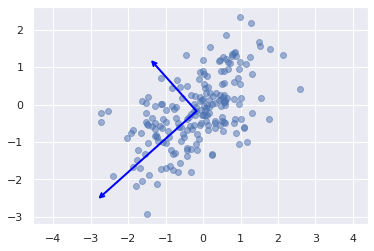
\includegraphics[width=0.75\textwidth]{pca}
\end{figure}

After you get the Principle Components, we project a user's data onto these axes.  This projection map can be called $\sum_i |e_i\rangle\langle u_i|$.  The $|e_i\rangle$ terms just say that we want the the $i$-th projection to go in the $i$-th coordinate.

\subsection{Normalization}

It's impossible to talk about PCA without discussing normalization.  Let's say you have two variables, age and annual income.  These things are likely correlated in your data, and you want to capture the best axis to capture these.  But age only varies between users by a couple of decades, whereas income varies by tens of thousands of dollars.  PCA will say that most of the variance lives with the variance on income.  But this doesn't actually make sense because income is measured in dollars and age is measured in years.  Our answer shouldn't change if we decide to measure income in Euros and age in minutes.  We need something unitless that captures some general sense of spread.  As well, the range of incomes will be different than the range of ages.  Why should a model capture that people don't get credit cards until the age of $18$?  We need something that also centers.

There are a few different ways to recenter and scale.  More generally such techniques are called regularization.  We'll take about a specific technique, call {\em normalization}.\footnote{Some readers will recognize the equation as the z-score used for normal distribution, from which normalization gets its name.}  This is done before we apply any algorithm.  For each variable $X$, with points $x_i$, we make new variables:

$$
x_i':=\frac{x_i-\operatorname{E}(X)}{\sqrt{\operatorname{Var}(X)}}
$$

Say that the $x_i'$ are points of the new variable $X'$.  Well mention some nice effects of normalization.  Subtracting the $\operatorname{E}(X)$ guarantees that $\operatorname{E}(X')=0$.  This is what allows us to ignore the $\operatorname{E}(X)^2$ in Eq. (\ref{var}) above.  We put a square root in the denominator (vs. using variance) to ensure that the unit matches the numerator.  Also notice that $\langle x_i'|(A')^TA'|x_i'\rangle=\frac{\langle x_i|A^TA|x_i\rangle}{\lambda_i^2} = \frac{\lambda_i^2}{\lambda_i^2}=1$.  Because the $\left\{|x_i\rangle\right\}$ form a basis, every vector in the span can be written as $|x\rangle=\sum_ia_i|x_i\rangle$, where $\sum_ia_i^2=1$; it follows that $\langle x|(A')^TA'|x\rangle=1$ for all $|x\rangle$.

\subsection{User embeddings}

Start with a matrix $A$ that maps users to their normalized features with SVD, $A=\sum_i|u_i\rangle\langle v_i|$.  (Notice:  The $\lambda_i=1$ because we normalized.)  We've been talking about principle components as the vectors $\left\{\vec u_i\right\}$.  But if we want to know the values for an actual user $e_j$, then we can first map the user to their raw variables, $A|e_j\rangle$.  Then project the raw values (number of bankruptcies, number of credit cards, etc.) onto the principle components by applying the map $\sum_{i=1}^{10}|u_i\rangle\langle u_i|$.  Then this equals:

$$
\left(\sum_{i=1}^{10}|e_i\rangle\langle u_i|\right)\left(\sum_{i=1}^{1000}|u_i\rangle\langle v_i|\right)|e_j\rangle = \sum_{i=1}^{10}|e_i\rangle\langle v_i|e_j\rangle
$$

Compare to the user embeddings from the last section, we get that the embedding of the $j$-th user with $10$ latent dimensions is $\sum_i|e_i\rangle\langle v_i|e_j\rangle$.  They're the same.  We might think of PCA as Collaborative Filtering, where we just don't use the embeddings of the features.  It's an imperfect analogy, because really these are used in different cases.  Not only do we not want the "embeddings" of the features, but the vectors $\left\{\vec u_i\right\}$ are not even meaningful in the same way that the movie vectors were; the rows of $U\sqrt D$ would be the embedding of a credit profile that has a single normalized feature set to $1$ and the rest set to $0$, which doesn't represent anything.

{\bfseries\scshape\Large Exercises}

\begin{enumerate}[\thechapter.\thesection .1]
\item \label{iris_pca} Load the Iris dataset.  In Python this can be done with:

\begin{lstlisting}
import sklearn.datasets
iris = sklearn.datasets.load_iris()
\end{lstlisting}

This is available in other languages too.  The dataset has $150$ datapoints with $4$ numerical features and a single categorical target.  In Python, you can get these as numpy arrays:

\begin{lstlisting}
features, target = iris["data"], iris["target"]
\end{lstlisting}

Use PCA to reduce the feature space to a $3$-dimensional space.  Report the principle components.  These should be three vectors, each $4$-dimensions.  You can either manually compute this using the SVD functionality introduced in Section \ref{computer_section}, or you can look up a PCA function (like in sklearn).
\item Given a matrix $A$, and an SVD $AA^T=UDV^T$, consider the embedding of the $i$-th row of $A$ given by $\sqrt DV^TA|e_i\rangle$.  Show that the dot product of the $i$-th embedding and the $j$-th embedding equals $\langle e_i|A^TDA|e_j\rangle$.
\item One might argue that the rows of the watch matrix from the previous section should be normalized.  What are some pros and cons of this?
\item $C=A^TA$ is sometimes called the covariance matrix, because every term, $C_{ij}$ is the covariance between the $i$-th and $j$-th variable.  Suppose $A'$ normalizes the rows of $A$.  Prove that $C'=(A')^TA'$ is a correlation matrix, in the sense that $C'_{ij}$ is the Pearson's correlation coefficient between the $i$-th and $j$-th variable of $A$.
\item For both parts of this problem, assume you have some matrix

$$
A=\left(\begin{array}{cc} x_1 & y_1 \\ x_2 & y_2 \\ \vdots & \vdots \\ x_n & y_n\end{array}\right)
$$

\begin{enumerate}
\item Suppose that for all $i$, $y_i=mx_i$ for some fixed $m$.  Prove that $A=\lambda|u\rangle\langle v|$, and that $|v\rangle$ spans all the data points $(x_i, y_i)$.  (Hint: Guess and verify an SVD, then observe that this is unique up to $\pm |v\rangle$.)
\item Suppose that for all $i$, $y_i=(m+\varepsilon_i)x_i$, where each $\varepsilon_i$ is taken independently from a normal distribution $\operatorname{N}(0, \sigma)$, for some small fixed $\sigma$.  Given an SVD, $A=\lambda_1|u_1\rangle\langle v_1|+\lambda_2|u_2\rangle\langle v_2|$, prove that $\operatorname{E}\left(|v_1\rangle\right)=|v\rangle$, where $|v\rangle$ is from part (a).
\end{enumerate}
\item Critique the following reasoning:  “A model is trained on a PCA based on 3 years worth of data.  After one month the PCA is updated with the extra month of data, but still using the first 3 years.  I shouldn’t have to retrain the model since the principle components will be approximately the same as the previous month.”
\end{enumerate}

\section{Partial Least Squares}

In the previous section, we may have rejected number of bankruptcies too quickly.  Though it's uncommon, it may be very predictive of a default.  If so, we should include it.  Instead of looking at variance of the feature space by itself, {\bf Partial Least Squares (PLS)}\footnote{Don't try to make sense of the name.} tries to find those axes that most correlate with the target.

Continuing the example, say that the target is loan default ($1$ for default and $0$ for no default).  We have historical data which says whether users with a given profile defaulted.  With $n$ historical data points, we put these targets in a $n\times 1$ matrix $X$.  We also have features for these data points, an $m\times n$ matrix $Y$.  $X^TY$ is a $1\times m$ matrix, where each entry $(X^TY)_{1j}$ is correlation coefficient of the $j$-th dimension of $Y$ with the target variable, provide that $X$ and $Y$ are normalized.  $\langle u|X^TY|v\rangle$ is the correlation between the axes $X|u\rangle$ and $Y|v\rangle$.  To maximize correlation, we find the maximizing $\vec u$ and $\vec v$, which we can again do with the SVD.  Of course, because $X$ is one dimensional, the only unit vector $|u\rangle$ (up to sign) is the singleton $(1)$.  The maximizing vector $|v\rangle$ is more interesting; it represents the axis in the feature space that most correlates with the target.  Because $X^TV$ will have rank $1$, we can only get a single PLS dimension out.  However, this dimension is likely to be a good dimension for predicting a default.

If there are multiple target dimensions, you could still perform an SVD on $X^TY$, and get as many PLS axes as there are target dimensions.  (See Exercise \ref{iris_pls} for an example of this.)  In that case, the vectors $\left\{\vec u_i\right\}$ will be non-trivial.  However, even in that case, only the dimensions in the feature space, $\left\{\vec v_i\right\}$ will be of interest.

Collaborative Filtering and PCA are considered {\bf unsupervised models}, because they don't take into account target.  PLS is a {\bf supervised model} because it does.  Unsupervised models are common for building embeddings, because we think of them as trying to capture some intrinsic about the data.  A single embedding will often be used in multiple applications, and tying too closely to a single target may not be desirable.

PLS is less commonly used than the other algorithms presented here.  One reason may be that it can only produce as many dimensions as you have targets.  (However, see Exercise \ref{pls_pca_ex} for a way to supplement PLS and PCA.)  Another reason may be that PCA is an unsupervised algorithm.  This means that you don't need target data.  But also, dimensionality reduction is usually done upstream of modeling; the output may be used for exploration or sent to many different applications.  A third reason that PLS is less common than PCA may just simply be that it is less well-known.  PLS might be thought of as a variant of PCA.  PCA is valued for its simplicity, and modelers probably don't spend much time researching variants.  In my experience, I've found that PLS can be very useful, especially if you have a single application in mind.  It's my opinion that PLS should be a tool in any modelers tool belt.

{\bfseries\scshape\Large Exercises}

\begin{enumerate}[\thechapter.\thesection .1]
\item \label{iris_pls} Load the Iris dataset.  (See Exercise \ref{iris_pca} for more details.)  Make three target variables, $1$ or $0$ indicating whether the datapoint is a Setosa, Versicolous, or Virginica iris.  Use PLS to reduce features to a $3$-dimensional space.
\item Critique the following model proposal:  "Given loan data, we use PLS to get the single dimension that is most correlated with default.  The applicants who score lower on this dimension must be less likely to default.  Approve all loans below a certain threshold."
\item You and a coworker are building an insurance model on credit data.  The model will be a logistic regression to predict the probability of an insurance claim.  You have historical claim data.  You think you should use only PLS, and your coworker thinks you should only use PCA.  How can you decide with data which model is better?
\item \label{pls_pca_ex} Consider a scheme where you use both PLS and PCA.  If you start with 1 PLS dimension $|x\rangle$, how can you choose the dimension that is orthogonal to this dimension and that captures the most variance?  That is, how do you find

$$
\max_{\left\||u_1\rangle\right\|=1, \langle x|u_1\rangle=0}\langle u_1|A^TA|u_1\rangle
$$
\item Imagine you fit a logistic regression on a PLS dimension.  Because the PLS dimension and the regression are both fit on the same data, you have concerns that you are overfitting the data.  How can you confirm that your model is not overfit?
\item Given a feature matrix, $\left(\begin{array}{cc}a&b\\c&d\end{array}\right)$, and a target variable, $\left(\begin{array}{c}x\\y\end{array}\right)$, suppose you compute a PLS dimension as $\left(\begin{array}{c}u\\v\end{array}\right)$.  Compute $\frac{\partial u}{\partial x}$, $\frac{\partial u}{\partial y}$, $\frac{\partial v}{\partial x}$, and $\frac{\partial v}{\partial y}$.
\item $\obot$ Start with embeddings from problem \ref{movie_lens_1} or found online, and filter this list to ~100 movies that people are likely to know.  (Look at the IMDB top 250 if you aren’t sure.)  Make a game, called Hot-or-Cold:  This game chooses a random (secret) game from the ~100 movies.  The user guesses which movie it is, and the program tells them how close they are to the target, by telling them the cosine similarity between the guessed movie and the secret movie.  Show the player the top 100 list, or allow the user to enter any movie from the larger dataset.
\end{enumerate}

\section{Canonical Correlation Analysis}

For this last section, we imagine that we’re making recommendations in the iPhone app store.  A partner team uses a model that takes as input features of apps that users have downloaded, and outputs a recommendation for a new app.  We don’t know exactly how that model works, but that team counts on us to build features that well represents apps.

We’ll consider a couple of good approaches to featurizing apps.  One approach is to use Collaborative Filtering to get co-download embeddings for the apps.  This means that if two apps have lots of users in common, then the apps’ embedding vectors will be near each other; apps with less users in common will be far apart.  Another approach is to use the app description.  These descriptions are entered by the developer and are presented to the user in the app store.  Somebody from the natural language team has made embeddings based on these text descriptions.

Although these two embeddings are capturing different signal, these signals are likely to be correlated.  For example, apps like Microsoft Teams, Microsoft Word, and Microsoft OneDrive are likely to be downloaded by the same people, but these are also likely to all say “Microsoft” in the description.  Here we think correlated signals may amplify each other.  The word “bird” might show up in bird watching apps, but also in bird-themed cell phone games (Angry Birds, Flappy Bird, and some knock-offs).  It’s not until a signal shows up in both embeddings that we think we’ve caught a family of related apps.

To do this, we look for axes that maximize covariance.  This is exactly the same problem as PLS.  Specifically, we start with two matrices of features $X$ and $Y$ of dimension $m_1\times n$ and $m_2\times n$, with $n$ the number of users, and $m_1$ and $m_2$ are the number of dimensions in the two feature sets.  The matrix $XY^T$ has entries $m_{ij}$ equal to the correlation between the $i$-th feature in $X$ and the $j$-th feature in $Y$.  We look for the axes that maximize $\langle u|XY^T|v\rangle$.  Again this is solved with an SVD.  We call the search for these axes a {\bf Canonical Correlation Analysis (CCA)}.

Many of the topics covered in this chapter are closely related, but none more than PLS and CCA.  Again the use cases for the two are much different.  For PLS, we use the target variable to determine the best axis among a single set of features.  But for CCA, we use two sets of features to find the best axis.

Because of this there are two sets of features, we end up having two signals to which we can attach for any user.  We can embed a user $|e_i\rangle$ by first mapping them to their $X$ features, then embedding this like we did in the Collaborative Filtering section, $\sqrt DU^TX|e_i\rangle$.  {\it Or} we could map first into $Y$ and embed, $\sqrt DVY^T|e_i\rangle$.  These are {\it almost} the same signal (see Exercise \ref{two_lsrl}), and in practice we could use just one of these signals.

{\bfseries\scshape\Large Exercises}

\begin{enumerate}[\thechapter.\thesection .1]
\item For each of the following scenarios choose one of the models we covered in this chapter, and describe how it could be used to help the situation.
\begin{enumerate}
\item Twitter is trying to recommend posts to users.  You have a lot of data about historical post views for each, and data about posts, including co-views and text embeddings.
\item You're trying to build a spam filter.  You have a large labeled set, and features for each of the emails, including text embeddings, domain-specific flags, and author information.
\item YouTube is trying to build a user embedding based on a very large number of features, including geographic, platform, demographics, watch history, and others.  The embeddings will be used for several applications.
\item Pinterest is trying to build a user embedding based only on what posts the user favorited.  The embeddings will be used for several applications.
\item An insurance company is trying to build a fraud detector based only on the text content of police reports.  You have a large number of labeled data points.
\end{enumerate}
\item \label{two_lsrl} You do CCA on two matrices $X$ and $Y$ to get that $XY^T=UDV^T$.  Imagine that we used the axes $\left\{\vec u_i\right\}$ to perform a linear regression.  A linear regression treats the vectors $\left\{\vec u_i\right\}$ as the data points, along with targets $y_i$, and it tries to find the coefficients that minimize the square error:

$$
\min_{\left\{c_j\right\}}\sum_i \left(y_i-\sum_jc_ju_{ij}\right)^2 = \min_{\langle c|}\sum_i \left(y_i-\langle c|u_{i}\rangle\right)^2
$$

\noindent Show that when $D=I$, that:

$$
\min_{\langle c|}\sum_i \left(y_i-\langle c|u_{i}\rangle\right)^2 = \min_{\langle c|}\sum_i \left(y_i-\langle c|v_{i}\rangle\right)^2
$$
\item Imagine you have two embeddings representing the same data.  To get a $20$-dimensional representation of the data, you suggest using CCA on the two embeddings.  Your coworker argues that to ensure orthogonality, you should instead do PCA on both embeddings individually to get $10$ dimensions from each.  How would you argue that your approach is better?
\item Suppose that $X$ and $Y$ have the same latent dimensions with different singular values.  That is, $X=\sum_i\lambda_i|u_i\rangle\langle v_i|$ and $Y=\sum_i\mu_i|u_i\rangle\langle v_i|$.  Show that the first axis that CCA produces is $\langle v_1|$.
\item Suppose that $X$ and $Y$ have SVDs $X=\sum_i\lambda_i^X|u_i^X\rangle\langle v_i^X|$ and $Y=\sum_i\lambda_i^Y|u_i^Y\rangle\langle v_i^Y|$, with $\langle u_i^X|v_j^Y\rangle=0$ and $\langle u_i^Y|v_j^X\rangle=0$ for all $i$ and $j$.  (The superscripts are indices, and not exponents.)  Prove that the resulting CCA axis are the principle components from $X$ and $Y$.  (Hint: Consider the PCA of $(X-Y)$.)
\end{enumerate}

\end{document}
